\cotefile{136}
\scanpage{235}
On considère l'anneau simplicial
\[
\widehat A_*^*(S,\gamma^*,t)^{\unsure{\wedge}}=\widehat A_*^{*\wedge}
\]
\unsure{par}
\[
\begin{aligned}
\widehat A_n^*&\simeq S\{\{X_0,\ldots,X_n\}\}/(\text{idéal }\inserted{\text{à p.d.}}\deleted{\text{\unsure{engendré}}}\inserted{\text{engendré par }\sum X_i-\unsure{t|\bar t}})\otimes_S\frac{\bigwedge^*[dX_0,\ldots,dX_n]}{\text{idéal }(\sum dX_i)}\\
(&\simeq S\{\{Y_0,\ldots,Y_{n-1}\}\}[dY_0,\ldots,dY_{n-1}]
\end{aligned}
\]
\deleted{$\simeq$}

On a donc
\[
\widehat A_*^*\simeq\widehat A_*^0\otimes_S\bigwedge^*\Psi_*^S.
\]
d'où
\[
\pi_\ell(\widehat A_*^i)=\pi_\ell(\widehat A_*^0\otimes\bigwedge^i\Psi_*^S)\simeq\pi_{\ell-i}(\widehat A_*^0)
\]
et il faut donc étudier $\pi_*(\widehat A_*^0)$.

On considère sur $\widehat A_*^0$ \deleted{$\unsure{\Gamma_S(\Phi_*)}$} la filtration décroissante par idéaux fermés stables par p.d. ``engendrée'' par la condition que \deleted{\unsure{pour}} \unsure{pour tout $n$}, les $X_i$ et $t$ sont en filtration $\geq1$. \unsure{On}
\[
\begin{aligned}
\mathrm{Fil}^0(\widehat A_n^0)&\simeq\deleted{\unsure{S}}\widehat A_n^0\\
\mathrm{Fil}^p(\widehat A_n^0)&\simeq\left\{\sum\deleted{\unsure{a}}a_{i_0\ldots i_n}\unsure{\big\{}X_0^{(i_0)}\cdots X_n^{(i_n)}\ \middle|\ a_{i_0\ldots i_n}\in S^{[p-\sum_0^n i_\alpha]}\right\}\\
&=\left\{\sum a_{i_0,\ldots i_{n-1}}Y_0^{(i_0)}\cdots Y_{n-1}^{(i_{n-1})}\ \middle|\ a_{i_0\ldots i_{n-1}}\in S^{\unsure{[p-\sum_0^{n-1}i_\alpha]}}\right\}.
\end{aligned}
\]
Bien sûr, la topologie \unsure{pr. div.} sur $\widehat A_n^0$ est aussi celle définie par cette filtration, et par suite $\widehat A_*^0$ est séparé et complet pour cette filtration. Un calcul immédiat donne, posant
\[
k=S/S^{[1]}
\]
\[
\mathrm{Gr}^p(\widehat A_*^0)\simeq\Gamma_k^p(\Phi_*^k)
\inserted{\simeq\widehat A_*^{p0}(\mathrm{Gr}^*(S),\widetilde\gamma^*,\widetilde t)}
\]
\margin{$\mathrm{Gr}^*(S)$ : $k$-\unsure{$\delta$}-algèbre graduée quotient de $k\unsure{\langle T\rangle|\{T\}}$.}
\inserted{si l'épi $k\unsure{\langle T\rangle|\{T\}}\longrightarrow\mathrm{Gr}^*(S)$ est un \uline{iso} \deleted{\unsure{et}} (donc $\mathrm{Gr}^p(\widehat A_*^0)$ flasque si $p\ne0$)}
d'où, dans cette hyp. \inserted{d'isomorphisme}
\[
\pi_i(\mathrm{Gr}^p(\widehat A_*^0))=\begin{cases}0&\text{si }p\ne0,\ i\ne0\ \deleted{\unsure{\longleftarrow}}\\k&\text{si }(i,p)=0\end{cases}
\]
d'où on conclut que \deleted{l'inclusion}
\[
\deleted{\mathrm{Fil}^1\widehat A_*^0\unsure{\hookrightarrow}\widehat A_*^0}
\]
\margin{234}
\scanpage{236}
- \mspage{188} - \margin{IX}
\[
\underline R_U/\underline R_U^{\mathrm f}\simeq M_U\ ,\tag{13.5.12}
\]
et l'homomorphisme $i$ de (13.3.4) peut s'écrire comme un homomorphisme
\[
i:M_U\longrightarrow A^{\unsure{\natural|\sharp}}\ ,\tag{13.5.13}
\]
qu'on retrouvera dans un contexte un peu différent au par. suivant.

14. \uline{Liens avec la théorie transcendante} : \uline{cas rigide-analytique}. \uline{L'homomorphisme canonique} $\underline M_K\longrightarrow A_K^{\unsure{\natural|\sharp}0}$.

14.1. Nous supposons connu ici les fondements de la théorie des espaces rigide analytiques, pour lesquels on pourra consulter [12] [13] [34].

Soit $S$ un trait complet, $A_K$ un schéma abélien sur son corps des fractions. On a construit alors dans 8.1, par descente à partir de l'extension de Raynaud dans le cas semi-stable, une extension $G_K=A_K^{\unsure{\natural|\sharp}0}$ (8.1.1)
\[
\text{(14.1.1)}\qquad
\diagram{\begin{tikzcd}0\arrow[r]&T_K\arrow[r]&G_K\arrow[r]&B_K\arrow[r]&0\end{tikzcd}}
\]
d'un schéma abélien $B_K$ par un tore $T_K$. Considérant le schéma abélien dual $A'_K$, on a de même une extension $G'_K=A_K'{}^{\unsure{\natural|\sharp}0}$
\[
\text{(14.1.2)}\qquad
\diagram{\begin{tikzcd}0\arrow[r]&T'_K\arrow[r]&G'_K\arrow[r]&B'_K\arrow[r]&0\end{tikzcd}}\ ,
\]
où $B'_K$ s'identifie d'ailleurs au schéma abélien dual de $B_K$ (8.2). On désigne, comme dans (8.1.8), par $\underline M_K$ et $\underline M'_K$ les réseaux sur $K$ duals de $T'_K$ et de $T_K$ respectivement :
\[
\underline M_K=D(T'_K)\ ,\qquad \underline M'_K=D(T_K)\ .\tag{14.1.3}
\]
\margin{235}
\margin{506}
\scanpage{237}
\deleted{On trouve donc
\[
H^i(C_{\mathrm{DR}}^*(X,\widehat A_*^*))=\begin{cases}H^0(X,S)&\text{si }i=0\\H^i(X,S^+)&\text{si }i\ne0.\end{cases}
\]}
\margin{\unsure{$*$}}
\[
\left\{\begin{aligned}
&\mathrm{Fil}^p(\widehat A_*^0)\text{ flasque pour tt }p\geq1\\
&\pi_i(\widehat A_*^0)=\begin{cases}0&\text{si }i\ne0\\k&\text{si }i=0\end{cases}\quad\text{si }p\leq0
\end{aligned}\right.
\]
Considérons la filtration d'algèbre \inserted{\unsure{simpliciale}} sur $\widehat A_*^*$ prolongeant celle de $\widehat A_*^0$ et donnant \deleted{\unsure{à}} à $\widehat A_*^1$ la filtration $1$, donc
\[
\mathrm{Fil}^p A_*^*=\sum_{0\leq i\leq p}\mathrm{Fil}^{p-i}(\widehat A_*^0)\otimes_S\bigwedge^i\unsure{\Psi_*^S|\Phi_*^S}
\]
\uline{C'est stable par l'opérateur différentiel}.
On a \deleted{\unsure{donc}}
\[
\begin{aligned}
\pi_\ell(\mathrm{Fil}^p(A_*^i))&=\deleted{\sum_{0\leq i\leq p}}\pi_\ell(\mathrm{Fil}^{p-i}(\widehat A_*^0)\otimes_S\bigwedge^i\Psi_*)\\
&\deleted{\unsure{=\pi_{\ell-i}(\mathrm{Fil}^{p-i}(\widehat A_*^0))}}\\
&=\pi_{\ell-i}(\mathrm{Fil}^{p-i}(\widehat A_*^0))\\
&=\begin{cases}0&\text{si }\deleted{\unsure{\ell\ne p\Longleftrightarrow i=p}}\ \unsure{\text{non }p\leq i\text{ et }\ell=i}\\k&\text{si }\deleted{\unsure{\ell-i=p}}\quad p\leq i=\ell\end{cases}
\end{aligned}
\]
\margin{\deleted{$\unsure{0\text{ si }\ell-i\ne p-i}$}\quad\deleted{$\unsure{\text{sinon }\ell=p}$}\quad\deleted{$\unsure{p-i\ne0\quad i\geq p}$}}

Donc \deleted{\unsure{on en conclut la suite spectrale (pour $p$ fixé)}} \deleted{$\unsure{E_2^{rs}=H^r(\mathcal H^s(X,S}$} si on regarde $\mathrm{Fil}^p(A_*^*)$ comme une résolution simpliciale de $\unsure{S_*^{[p]}}=\mathrm{Fil}^p S$, on voit que tous les termes $\mathrm{Fil}^p(A_*^i)$ de cette résolution \inserted{en degré $<p$} sont flasques, \deleted{\unsure{tandis que}} \deleted{\unsure{le premier}} \deleted{\unsure{terme}} $(j\geq p)$ $\mathrm{Fil}^p(A_*^j)\simeq\widehat A_*^0\otimes_S\bigwedge^j\Psi_*$ dont le seul gpe d'homotopie non nul est $\pi_j(\cdot)\simeq k$. On en conclut
\[
\diagram{\begin{tikzcd}[column sep=large,row sep=large]
H^i(\mathrm{Fil}^p C_{\mathrm{DR}}^*(X,\widehat A_*^*))\arrow[r,"\simeq"]\arrow[d]&H^i(X,\underset{\mathrm{Fil}^pS}{\underbrace{S^{[p]}}})\arrow[d]\quad\text{si }i\leq p\\
H^{\unsure{i}}(C_{\mathrm{DR}}^*(X,\widehat A_*^*))\arrow[r]&H^i(X,S)
\end{tikzcd}}
\]
\inserted{\unsure{ou déf.} $(C_{\mathrm{DR}}^*(X,\mathrm{Fil}^p\widehat A_*^*))$}
\margin{236}
\scanpage{238}
- \mspage{186} - \margin{IX}
\[
{}_n A^0\simeq\underline R\otimes_{\mathbb Z}\mathbb Z/n\mathbb Z\ ,\tag{13.5.5}
\]
qui donne, pour $n$ parcourant les puissances d'un nombre premier $\ell$ donné, un isomorphisme de systèmes projectifs de groupes sur $S$
\[
T_\ell(A^0)\simeq\underline R\otimes_{\mathbb Z}\mathbb Z_\ell\ ,\tag{13.5.6}
\]
où $\mathbb Z_\ell$ est considéré comme le système projectif des $\mathbb Z/\ell^{n+1}\mathbb Z$. Dans le cas envisagé ici où $A$ provient d'un schéma en groupes séparé sur $S$, on voit alors immédiatement que les $\underline R\otimes\mathbb Z/n\mathbb Z$ peuvent être considérés comme des schémas relatifs, ce qui donne un sens au symbole $(\underline R\otimes_{\mathbb Z}\mathbb Z_\ell)_{\underline{\unsure{O|0}}}$ (alors que $R_{\underline{\unsure{O|0}}}$ n'en aurait pas en général !), et on obtient un isomorphisme canonique
\[
T_\ell(A_{\underline{\unsure{O|0}}})\unsure{\overset{?}{\simeq}|\simeq}(\underline R\otimes_{\mathbb Z}\mathbb Z_\ell)_{\underline{\unsure{O|0}}}\ .\tag{13.5.7}
\]
Il résulte alors immédiatement des constructions du par. 2 et de 13.3 que l'isomorphisme précédent transforme partie fixe en partie fixe, partie torique en partie torique :
\[
T_\ell(A_{\underline{\unsure{O|0}}})^{\mathrm f}\simeq(\underline R^{\mathrm f}\otimes_{\mathbb Z}\mathbb Z_\ell)_{\underline{\unsure{O|0}}}\ ,\quad T_\ell(A_{\underline{\unsure{O|0}}})^{\mathrm t}\simeq(\underline R^{\mathrm t}\otimes_{\mathbb Z}\mathbb Z_\ell)_{\underline{\unsure{O|0}}}\ .\tag{13.5.8}
\]
Si $A'$ est un groupe analytique relatif sur $S$ satisfaisant aux mêmes hypothèses que $A$, et si $W_{\underline{\unsure{O|0}}}$ est une biextension de $(A_{\underline{\unsure{O|0}}},A'_{\underline{\unsure{O|0}}})$ par $\mathbb G_{m\underline{\unsure{O|0}}}$, définissant donc au-dessus d'un voisinage de $s$ une biextension de $(A,A')$ par $\mathbb G_{mS}$ (en travaillant maintenant avec la notion au sens analytique complexe, obtenue en travaillant dans le site des espaces analytiques au-dessus de $S$, pour une topologie convenable \ldots), alors d'après VIII 2.2 $W$ définit des accouplements
\margin{504}
\margin{237}
\margin{504}
\scanpage{239}
qui s'écrit aussi
\[
\diagram{\begin{tikzcd}[column sep=large,row sep=large]
H^i(\mathrm{Fil}^p C_{\mathrm{DR}}^*(X;S,t,\gamma^*))\arrow[r,"\sim"]\arrow[d]&H^i(X,\mathrm{Fil}^pS)\arrow[d]\\
H^i(\mathrm{Fil}^q C_{\mathrm{DR}}^*(X;S,t,\unsure{\gamma'|\gamma^*}))\arrow[r]&H^i(X,\mathrm{Fil}^qS
\end{tikzcd}}
\]
\margin{$q\leq p$}
\margin{\figure{\begin{tikzpicture}\node[draw,ellipse] {\uuline{Iso si}};\end{tikzpicture}} \uuline{$i\leq p$}}
\margin{\uline{iso} si $i\leq q$}

\uline{NB} Si on ne suppose pas que l'épi
\[
k\{T\}\longrightarrow\mathrm{Gr}^*(S)
\]
est un iso, on ne peut rien dire. Prenons p.ex. le cas extrême de dégénérescence
\[
t=0,\quad\text{donc }S\xrightarrow{\sim}k
\]
on a alors
\[
\mathrm{Gr}^p\widehat A_*^{\unsure{0}}\simeq\Gamma_k^p(\Psi_*)\ .
\]
donc
\[
\mathrm{Gr}^p(\widehat A_*^{\unsure{0}})\simeq\unsure{\Pi_*|K_*}(k,p)
\]
qui n'est flasque pour aucun $p\geq0$ (si $k\ne0$).

Prenons aussi le cas de $(\mathbb Z_p,p)$, la pd-filtration définie par $p$ est cofinale à la filtration $p$-adique si $p\ne2$ (si $p=2$, c'est la filtration constante de valeur
\[
\mathrm{Fil}^{\unsure{r|p}}\mathbb Z_2=2\mathbb Z_2\text{ si }\unsure{r|p}\geq1,\quad\text{donc}\quad\mathrm{Gr}^*(S)\simeq\mathrm{Gr}^0(S)\simeq\mathbb F_2
\]
dans ce cas, i.e. c'est encore le cas de dégénérescence\ldots), quel est exactement l'idéal $S^{[i]}$ engendré par les $\dfrac{p^j}{j!}$ pour $j\geq i$ ?
\margin{\deleted{$\unsure{S^{[i]}=(\frac{p^n}{n!}\mathbb Z_p)}$}\deleted{\unsure{--- i.e. quelle}}}
\deleted{\unsure{i.e. quelle est}}
\margin{238}
\scanpage{240}
- \mspage{185} - \margin{IX}
phisme (i.e. tel que $\underline O_S\longrightarrow f_*(\underline O_{S'})$ soit injectif) est un \uline{morphisme de descente effective} pour la catégorie fibrée des schémas abéliens relatifs.

b) Il semble que la méthode de démonstration de 13.5.2 doive permettre aussi de prouver le résultat analogue pour tout espace analytique $B$ propre sur $S$. Plus délicate sans doute est la question de savoir si, pour un espace analytique $X$ propre sur $S$, tel que le complété formel $\widehat X$ le long de $X_s$ soit algébrisable, $X$ est algébrisable sur $S$ au voisinage de $s$. Signalons seulement qu'il y a lieu ici de prendre la notion d'algébrisabilité relative de $X$ sur $S$ dans un sens plus large que dans [10], en entendant par là qu'au voisinage de $s$, $X$ provient d'un \uline{espace algébrique} sur $\underline O_{S,s}$ au sens de M. ARTIN [1].

13.5.4. Plaçons-nous dans les conditions de 13.5.1. Choisissons par ailleurs, pour tout entiers $n>0$, l'isomorphisme standart de groupes sur $\mathbb C$
\[
\mu_{n\mathbb C}\simeq(\mathbb Z/n\mathbb Z)_{\mathbb C}\ ,\quad m\longmapsto\exp(2i\pi m/n)\ ,
\]
ce qui nous donne, par passage à la limite sur les puissances d'un nombre fixé $\ell$, un isomorphisme canonique de faisceaux $\ell$-adiques sur $\mathbb C$ :
\[
\mathbb Z_\ell(1)_{\mathbb C}\simeq\mathbb Z_{\ell\mathbb C}\ ,
\]
que nous utiliserons pour identifier les deux membres.

De la suite exacte (13.1.3), on déduit, en appliquant la suite exacte des $\underline{\mathrm{Ext}}_{\mathbb Z}^i(\mathbb Z/n\mathbb Z,-)$, un isomorphisme canonique
\margin{\unsure{503|502}}
\margin{239}
\margin{503}
\scanpage{241}
\[
\nu_p(n!)=\frac1{p-1}(n-\mathrm{chiff}_p n)
\]
\[
\nu_p(p^{(n)})=\nu_p\left(\frac{p^n}{n!}\right)=\frac1{p-1}\bigl((p-2)n+\uline{\mathrm{chiff}_p n}\bigr)\quad(=\mathrm{chiff}_p(n)\text{ si }p=2)
\]
\deleted{\unsure{Si on}}
\[
\begin{aligned}
\gamma_{p,i}&=\mathop{\mathrm{Inf}}_{\uline{n\geq i}}\nu_p(p^{(n)})=\mathop{\mathrm{Inf}}_{\uline{n\geq i}}\frac1{p-1}\underbrace{((p-2)n+\mathrm{chiff}_p(n))}_{\text{cette fonction en }n\text{ n'est ni croissante ni décroissante}\ldots}\\
&=\begin{cases}1&\text{si }p=2\\>\dfrac{p-2}{p-1}i\underset{i\to+\infty}{\longrightarrow}+\infty&\text{si }p\ne2\end{cases}
\end{aligned}
\]
\[
i=i_0+i_1p+\cdots+i_rp^r
\]
\deleted{\unsure{disons}}
\margin{\deleted{$i_0$}\quad\deleted{$\unsure{i}$}}
\[
\underbrace{\underbrace{(p-1)}_{i_0}+\cdots+\underbrace{(p-1)p^{s-1}}_{i_{s-1}}}_{\unsure{p^{s+1}-1|p^s-1}}+\underset{\unsure{<p-1}}{\underbrace{i_s}}p^{\unsure{s}}+\cdots+i_rp^r
\]
\[
i+1=\unsure{i_s+1|i_s}\,p^{\unsure{s}}+\cdots+i_rp^r
\]
\[
(p-2)i+(p-1)\unsure{s}\deleted{\unsure{0}}+\deleted{\sum_{\alpha\geq s}i_\alpha}\leq(p-2)(i+1)+\deleted{\sum_{\alpha\geq s}\unsure{i'_\alpha|i_\alpha}}
\]
\[
[\nu_p(p^{(i)})\leq\nu_p(p^{(i+1)})]\Longleftrightarrow[(p-1)s\leq(p-2)]\Longleftrightarrow[s=0]\Longleftrightarrow[i_0\ne p-1]
\]
\[
\deleted{\boxed{i_0\leq p-2}}\Longleftrightarrow i+1\not\equiv0\ (p)
\]
Exemple \unsure{où|si} $\gamma_{p,i}=\gamma_{p,i+1}$ : il \uline{suffit} qu'on ait \deleted{$\unsure{\nu_p(p)}$}
\[
\nu_p(p^{(i+1)})\leq\nu_p(p^{(i)})
\]
i.e. que \deleted{\unsure{dans le cas}} \deleted{\unsure{pour le cas}} $i+1\equiv0\ (p)$,
i.e. $i$ de la forme $p\ell-1$
\margin{240}
\scanpage{242}
- \mspage{182} - \margin{IX}
13.5. \uline{Cas d'une situation relativement algébrique}. Nous supposons maintenant que $A$ provient d'un schéma en groupes relatif sur $S$, lisse, séparé et à fibres des extensions de schémas abéliens par des tores. Nous désignerons ce schéma relatif par la même lettre $A$. (Nous nous autorisons cet abus de notation grâce au fait que le foncteur $G\longmapsto G^{\mathrm{an}}$, qui va de la catégorie des schémas en groupes relatifs du type envisagé vers la catégorie des groupes analytiques sur $S$, est pleinement fidèle, comme il serait facile à établir grâce aux résultats du type GAGA relatifs [10].) Pour tout ce qui concerne la notion de schéma relatif, et les relations entre schémas relatifs sur $S$ et espaces analytiques sur $S$, nous renvoyons à [10] (cf. aussi [2, Exp. 15]). Si $\underline O$ désigne l'anneau local de $S$ en $s$, le schéma relatif $A$ est connu au voisinage de $s$ par la connaissance du schéma ordinaire $A_{\underline O}$ sur $\operatorname{Spec}(\underline O)$, déduit de $A$ par localisation en $s$. Il est clair alors que le complété formel de $A_{\underline O}$ le long de sa fibre spéciale (isomorphe à $A_s=A_0$) est isomorphe au complété formel du groupe analytique $A$ le long de $A_s$ (13.2), en identifiant les $A_n=A\times_S S_n$ à des schémas algébriques sur $S$, par l'abus de notations introduit ci-dessus. Dans le cas favorable où $\widehat A$, regardé comme schéma formel en groupes sur $\widehat{\underline O}$, est algébrisable (7.2.1), ce qui est le cas en particulier si $S$ est normal en $s$ et $A$ quasi-projectif sur $S$ (7.1.5) on obtient donc un schéma en groupes $A_{\widehat{\underline O}}^{\unsure{\natural|\sharp}}$ sur $\operatorname{Spec}(\widehat{\underline O})$, extension d'un schéma abélien $B_{\widehat{\underline O}}$ par un tore. Pour simplifier, nous supposons que $B_{\widehat{\underline O}}$ est projectif sur $\widehat{\underline O}$ (ce qui est bien le cas, on le sait, si $\underline O$ donc $\widehat{\underline O}$ est normal). On va alors prouver :
\margin{\unsure{1}}
\margin{500}
\margin{241}
\margin{500}
\scanpage{244}
\margin{\figure{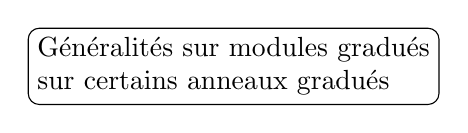
\begin{tikzpicture}\node[draw,rounded corners,align=left] {Généralités sur modules gradués\\sur certains anneaux gradués};\end{tikzpicture}}}
$S$ anneau $\mathbb Z$-gradué \unsure{comm.} à degrés $\geq0$
\[
S^0=k
\]
$\mathcal M$ catégorie des $S$-modules gradués

\figure{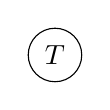
\begin{tikzpicture}\node[draw,circle] {$T$};\end{tikzpicture}} foncteur translation : $T(M)_n=M_{n+1}$
\margin{\figure{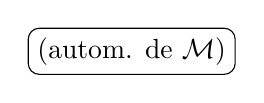
\begin{tikzpicture}\node[draw,rounded corners] {(autom. de $\mathcal M$)};\end{tikzpicture}}}
$T^i$ itéré $i$-ème $(i\in\mathbb Z)$\qquad $T^i(M)_n=M_{n+i}$
\[
\textcircled{$\mathcal M^+$}\subset\mathcal M\quad\big|\quad S\text{-modules gradués à degrés }\geq0
\]
N.B. $\boxed{T^{-1}(\mathcal M^+)\subset\mathcal M_+}$
\[
T^{\unsure{-N}}(\mathcal M^+)=\unsure{\mathcal M_N|\mathcal M_N^*}\qquad S\text{-modules gradués à degrés }\geq N
\]
$(\mathcal M_0=\mathcal M^+)$
\[
N\leq N'\Longrightarrow\mathcal M_N\supset\mathcal M_{N'}
\]
\deleted{$\unsure{\mathcal M}$}
$\mathcal N=$ catégorie des $k$-modules (pas gradués)
\[
M_0\longrightarrow M_0\otimes_kS
\]
\[
\figure{\begin{tikzpicture}\node[draw,ellipse] {$\boxed{\mathcal N\xrightarrow{\varphi}\mathcal M}$};\end{tikzpicture}}\quad\text{se factorise par }\mathcal M^+=\mathcal M_0
\]

\textcircled{1} Étude de l'inclusion (pl. fid.)
\[
\mathcal M_{N'}\underset{i_{N,N'}}{\hookrightarrow}\mathcal M_N\qquad N'\geq N
\]
Commute aux $\varinjlim$ et $\varprojlim$, donc on s'attend à trouver des adjoints à g. et à dr.

\uline{Adjoint à droite} \inserted{$\tau_{N',N}$} \uline{de} $i_{N,N'}$
\[
\tau_{N',N}:\mathcal M_N\longrightarrow\mathcal M_{N'}
\]
\[
\tau_{N',N}(M)_i=\begin{cases}0&\text{si }i<N'\\M_i&\text{si }i\geq N'\end{cases}
\]
C'est un \uline{sous-module} de $M\in\operatorname{Ob}\mathcal M_N$
(car $S$ à degrés $\geq0$)
\margin{\deleted{MATHÉMATIQUES}\par\deleted{PROFESSEUR}\par\deleted{M. GROTHENDIECK ALEXANDRE}\par\deleted{5-856}}
\margin{243}
\scanpage{245}
% The printed letter is upside down in the supplied scan; reading order follows the upright letter.
Le Professeur Pierre, Robert LAFON\\
Directeur de l'U.E.R. IX\\
de l'Université Paul Valéry\\
--------

Montpellier, le 20 mai 1975

LE QUEBEC ``C''\\
Avenue des Etats du Languedoc\\
34000 MONTPELLIER

\margin{\illegible{1}}
à\\
Monsieur le Directeur\\
de l'U.E.R.\\
de l'Université\\
de Montpellier

Monsieur le Directeur et Cher Collègue,

Comme vous le savez, une Université du 3ème Age a été créée dans l'U.E.R. IX de l'Université Paul Valéry.

Après trois mois d'expérience, il s'avère que cette création correspond à un besoin de la population, puisque plus de ``500 étudiants'' fréquentent les diverses activités entreprises au cours de cette année expérimentale. Nous devons nous attendre à un effectif plus important à la prochaine rentrée universitaire, aussi, je serais désireux de multiplier les enseignements et je vous serais reconnaissant si vous pouviez demander aux Collègues de votre U.E.R., s'ils accepteraient éventuellement de participer à cet enseignement et de me faire des propositions, afin qu'en accord avec les étudiants du 3ème Age, nous puissions mettre sur pied le programme de l'année 75/76.

Ces enseignements peuvent être faits, sous forme de conférences magistrales isolées, d'heures de cours hebdomadaires ou mensuels, ou de sessions intensives. Il peut y avoir également des visites organisées ou des activités pratiques.

Sans doute, je pourrais faire appel au bénévolat, mais je pense qu'il est plus convenable d'honorer selon les règles de l'Education Nationale, les collègues qui accepteraient de participer à ces enseignements.

Je vous serais reconnaissant de diffuser cette lettre aux membres de votre U.E.R., en demandant à nos collègues une réponse assez rapide, soit par lettre, soit en prenant contact avec moi, directement à mon domicile, par téléphone, au 58.24.50, de préférence en début d'après midi.

Je vous remercie de l'aide que vous voudrez bien m'apporter dans le développement de cette Université et vous prie de croire, Monsieur le Directeur et cher Collègue, à l'expression de mes sentiments les plus dévoués.

Diffusion : Liste B - n° 3211

Transmis pour information\\
et suite à donner.

Les Directeurs d'U.E.R. d'Enseignement

\unsure{R. Lafon}
\figure{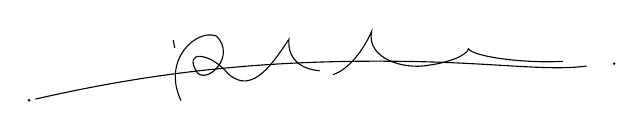
\begin{tikzpicture}[x=1cm,y=1cm]
\draw (0,0) .. controls (1.4,.32) and (2.8,.5) .. (4.6,.48) .. controls (5.8,.47) and (6.5,.35) .. (7,.42);
\draw (1.85,-.02) .. controls (1.6,.5) and (2.05,.9) .. (2.3,.8) .. controls (2.55,.55) and (2.2,.2) .. (2.06,.33) .. controls (1.86,.63) and (2.22,.6) .. (2.45,.32) .. controls (2.76,.04) and (3.03,.48) .. (3.22,.76) .. controls (3.2,.5) and (3.38,.38) .. (3.61,.36);
\draw (3.78,.31) .. controls (3.98,.38) and (4.16,.61) .. (4.27,.86) .. controls (4.2,.52) and (4.67,.37) .. (4.99,.43) .. controls (5.23,.46) and (5.48,.55) .. (5.5,.64) .. controls (5.55,.54) and (6.21,.45) .. (6.7,.48);
\draw (1.77,.65)--(1.75,.75);\fill (7.35,.45) circle (.018);\fill (-.08,-.015) circle (.018);
\end{tikzpicture}}
Pr P.R. LAFON
\margin{244}
\scanpage{246}
\[
\tau_{N',N}(M)\hookrightarrow M
\]
Soit $M\in\operatorname{Ob}\mathcal M_N$, $\unsure{P}\in\operatorname{Ob}\mathcal M_{N'}$,
\[
\diagram{\begin{tikzcd}[column sep=large]
\operatorname{Hom}_{\mathcal M_N}(i_{N,N'}(P),M)\arrow[d,equal]&\operatorname{Hom}_{\mathcal M_{N'}}(P,\tau_{N',N}(M))\arrow[l,"\sim"']\arrow[d,equal]\\
\operatorname{Hom}_{\mathcal M}(P,M)&\operatorname{Hom}(P,\tau_{N',N}(M))\arrow[l,"\sim"']
\end{tikzcd}}
\]
\uline{Adjoint à gauche} $q_{N',N}$ \uline{de} $i_{N,N'}$
\[
\diagram{\begin{tikzcd}[column sep=large]
\operatorname{Hom}_{\mathcal M_N}(M,i_{N,N'}(\unsure{P}))=\arrow[d,equal]&\\
\operatorname{Hom}_{\mathcal M}(M,P)\arrow[r,equal]&\operatorname{Hom}_{\mathcal M}(M/\substack{\text{ss.-module}\\\text{engendré par}\\\text{les }M_i,\ i<N'},P
\end{tikzcd}}
\]
\[
\diagram{\begin{array}{cccccccccc}
0&0&M_N&M_{N+1}&M_{N+2}&\cdots&M_{N'-1}&M_{N'}&M_{N'+1}&\cdots\\
0&0&0&&0&\cdots&0&\unsure{P}_{N'}&\unsure{P}_{N'+1}&\cdots
\end{array}}
\]
\[
q_{N',N}(M)=M/\substack{\text{ss.-module de }M\text{ engendré}\\\text{par les }M_i,\ i<N'}
\]
\uline{NB} $q_{N',N}$ et $\tau_{N',N}$ sont des ``foncteurs de localisation'' (car \unsure{adjoints} d'un foncteur pl. fid.);
\deleted{et} $q_{N',N}$ est exact à droite (en fait, commute aux $\varinjlim$ \unsure{quelc.}) mais en général pas à gauche, sans doute --- on ne s'attend pas qu'il ait encore un adj. à g. Par contre $\tau_{N',N}$ commute aux $\varprojlim$ \uline{et} aux $\varinjlim$ (à fortiori il est exact). On s'attend à en trouver un foncteur adjoint à droite.
\margin{$q_{N',N},\ i_{N,N'},\ \tau_{N',N}$}
\margin{245}
\scanpage{247}
\deleted{
\[
\diagram{\begin{tikzcd}[column sep=small,row sep=small]
A^*&\cdot\arrow[d,dash]&d\arrow[d,dash]&J\arrow[dr,dash,bend right=15]&\gamma\arrow[dd,dash,bend right=30]\quad\deleted{\unsure{\text{p.d.}}}\\
\substack{\circledast\ \text{groupe gradué}\\\text{à degrés }\geq0}&\substack{\circledast\ \text{multiplication}\\\text{associative}\\\text{unitaire}\\\uline{1\in A^0}}&\substack{\circledast\ \text{différentielle}\\d^2=0}&&\text{Sous-groupe}\\
&&&&\substack{\circledast\ \text{puissances divisées sur }J}
\end{tikzcd}}
\]
$\circledast$\ alg. graduée
\[
x\in A^i,\ y\in A^j\Longrightarrow xy\in A^{i+j}
\]
alg. comm., i.e.
\[
\left\{\begin{aligned}xy&=(-1)^{ij}yx\\x^2&=0\quad\text{si }x\in A^i,\ i\text{ impair.}\end{aligned}\right.
\]
$\circledast$\ $d$ de degré $+1$

$\circledast$\ $d(xy)=(dx)y+(-1)^{\deg x}x\,dy$

$\circledast$\ contient $A^+=\sum_{i>0}A^i$, donc \deleted{gradué} \inserted{de la forme} $J^0+\sum_{i>0}A^i$

$\circledast$\ idéal (i.e. gr. idéal)

$\circledast$\ stable par $d$ (automatique)

\deleted{$x^{(\alpha)}=0$}

$\circledast$\ $x\in A^i\Longrightarrow x^{(\alpha)}\in A^{\alpha i}$

$\circledast$\ \deleted{$d(x^{\alpha})=$}
\[
x\in\sum_{i\ \mathrm{imp}}A^i,\quad\deleted{\unsure{i\text{ pair}}},\quad\alpha\geq2\Longrightarrow x^{(\alpha)}=0
\]
\inserted{$\unsure{x_i\in A^{\mathrm{imp}}},\ y_i\in A$}

$\circledast$\ $d x^{(\alpha)}=x^{(\unsure{\alpha-1|\alpha+1})}dx$

\deleted{$\unsure{A_+^0}$}
\[
A^{\mathrm{pair}}+A^{\mathrm{impair}}=A^0+A^1
\]
\[
J^0\quad\unsure{-}
\]
\[
\left(\sum_{i\ \mathrm{pair}}x_i+\sum_{j\ \mathrm{impair}}y_j\right)^\alpha
\]
\[
A^0+A^1\quad\deleted{\unsure{\text{commut.}}}
\]
\deleted{$\unsure{(\sum x\,y=\sum x_i y+)}$}
\[
\deleted{(x+y)^2=x^2+y^2+xy+yx}
\]
\[
A^0\cdot A^1\subset A^1,\quad A^1 A^1\subset A^0
\]
\[
\bigwedge^2 A^1\unsure{\longrightarrow|-}\unsure{\overline A^0|A^0}\subset A^0
\]
\[
J^0+A^1=J\qquad\underset{\substack{x\in J^0\\y\in A^1}}{\unsure{\Downarrow}}
\]
\[
(x+y)^{(\alpha)}=\deleted{\sum}x^{(\alpha)}+x^{(\alpha-1)}y+\deleted{x^{(\alpha-2)}y^{(2)}}\ \unsure{\cdots}\qquad\deleted{(x+y)^2}
\]
\[
z^{(\alpha)}=(\deleted{x+y})^{(\alpha)}=x^{(\alpha)}+x^{(\alpha-1)}y
\]
\[
z'{}^{(\alpha)}=(x'+y')^{(\alpha)}=x'{}^{(\alpha)}+x'{}^{(\alpha-1)}y'
\]
\deleted{$(x+x')$}
\[
\begin{aligned}
(z+z')^{(\alpha)}&=((x+x')+(y+y'))^{(\alpha)}=(x+x')^{(\alpha)}+(x+x')^{(\alpha-1)}(y+y')\\
&=\sum_{i+j=\alpha}x^{(i)}x'{}^{(j)}+\left(\sum_{i+j=\alpha-1}x^{(i)}x'{}^{(j)}\right)(y+y')
\end{aligned}
\]
\unsure{Or}
\[
\begin{aligned}
\sum_{i+j=\alpha}z^{(i)}z'{}^{(j)}&=\sum_{i+j=\alpha}(x^{(i)}+x^{(i-1)}y)(x'{}^{(j)}+x'{}^{(j-1)}y')\\
&=\sum_{i+j=\alpha}x^{(i)}x'{}^{(j)}+\left(\sum_{i+j=\alpha-1}x^{(i)}x'{}^{(j)}\right)(y+y')\\
&\qquad+\left(\sum_{i+j=\alpha-2}x^{(i)}x'{}^{(j)}\right)yy'
\end{aligned}
\]
\[
\boxed{\text{OK si }yy'=0}
\]
}
\margin{246}
\scanpage{248}
D'ailleurs $\tau_{N',N}$, étant un foncteur de localisation exact, commutant aux $\varinjlim$, est un foncteur de passage au quotient modulo une ss-catégorie abélienne épaisse stable par $\varinjlim$ --- à savoir la sous-catégorie des $M$ \deleted{\unsure{\{} } tels que \deleted{$\unsure{M_0}$} $(\tau_{N',N}M=0\text{ i.e.})$ $M_i=0$ pour $i\geq N'$.

\uline{Adjoint à droite} $\rho_{N,N'}$ \uline{de} $\tau_{N',N}$
\[
\diagram{\begin{tikzcd}[column sep=large,row sep=large]
\operatorname{Hom}_{\mathcal M_{N'}}(\tau_{N',N}(M),P)\arrow[r,"\overset{?}{\sim}"]\arrow[d,equal]&\operatorname{Hom}_{\mathcal M_N}(M,\rho_{N,N'}P)\\
\operatorname{Hom}_{\mathcal M}(\tau_{N',N}(M),P)\arrow[d,phantom,"\cap" description]&\\
\displaystyle\prod_{i\geq N'}\operatorname{Hom}_k(M_i,P_i)&
\end{tikzcd}}
\]
\[
\diagram{\begin{tikzcd}[column sep=small,row sep=small]
0&0&M_N&M_{N+1}&\cdots&M_{N'-1}&M_{N'}\arrow[d]&M_{N'+1}\arrow[d]&\cdots\\
0&0&0&0&&0&P_{N'}&P_{N'+1}&\cdots
\end{tikzcd}}
\]
\deleted{
\[
\rho_{N,N'}(P)_i=\left\{\begin{aligned}&\unsure{P_i}\quad\unsure{i\geq N'}\\&\unsure{\subset}\ \unsure{\prod_{j\geq N'-i}\operatorname{Hom}_{k_0}(S_j,P_{i+j})}\end{aligned}\right.
\]
\[
\unsure{\operatorname{Hom}_{\mathcal M}(T^{-i}\tau_{N'-i,0}\underbrace{S}_{\in\mathcal M_{N'}},P)}
\]
\[
\unsure{\simeq\operatorname{Hom}_{\mathcal M}^{i}(\tau_{N'-i,0}(S),P)}
\]
}
\[
\begin{aligned}
\rho_{N,N'}(P)_i&=\begin{cases}0&\text{si }i<\unsure{N|N'}\\\operatorname{Hom}_{\mathcal M}^i(\tau_{\unsure{N'-i}}S,P)\end{cases}\\
&\simeq\operatorname{Hom}_{\mathcal M_N}(T^{-i}\tau_{N'-i}S,P)\qquad\text{si }i\geq N
\end{aligned}
\]
\margin{247}
\scanpage{249}
\margin{248}
\deleted{
\[
(\lambda z)^{(\alpha)}\overset?=\lambda^\alpha z^{(\alpha)},
\qquad \underset{A\ \uparrow}{\lambda}\quad\underset{J\ \uparrow}{z}.
\qquad
\left(\sum_{i\ \unsure{\mathrm{pair}|\mathrm{impair}}}x_i\right)
\left(\sum_{j\ \mathrm{impair}}y_j\right)=\sum_{i,j}x_i y_j.
\]
\[
\lambda=\underset{A^0\ \uparrow}{\unsure{\zeta|\xi}}+
\underset{A^1\ \uparrow}{\eta},\qquad z=x+y.
\]
\[
\lambda z=\underset{A^0\ \uparrow}{(\zeta x+\eta y)}+
(\zeta y+\underset{x\eta}{\uline{\eta x}}).
\]
\[
\begin{aligned}
(\lambda z)^{(\alpha)}
 &= (\zeta x+\eta y)^{(\alpha)}
 +(\zeta x+\eta y)^{(\alpha-1)}(\zeta y+x\eta)\\
 &=\sum_{\unsure{i+j=\alpha}}(\zeta x)^{(i)}(\eta y)^{(j)}
 +\left(\sum_{i+j=\alpha-1}(\zeta x)^{(i)}(\eta y)^{(j)}\right)
 (\zeta y+x\eta).
\end{aligned}
\]
\[
\begin{aligned}
\lambda^\alpha z^{(\alpha)}
 &=(\zeta^\alpha+\alpha\zeta^{\alpha-1}\eta)
 (x^{(\alpha)}+x^{(\alpha-1)}y)\\
 &=(\zeta^\alpha x^{(\alpha)}+
 \alpha\unsure{\zeta^{\alpha-1}}x^{(\alpha-1)}\eta y)
 +(\zeta^\alpha x^{(\alpha-1)}y+
 \overbrace{\alpha\zeta^{\alpha-1}x^{(\alpha)}}^{\unsure{\zeta^{\alpha-1}}}\eta)\\
 &=\bigl((\zeta x)^{(\alpha)}+\alpha(\zeta x)^{(\alpha-1)}(\eta y)\bigr)
 +\bigl(\zeta(\zeta x)^{\unsure{\alpha-1|(\alpha-1)}}y+
 x(x\zeta)^{(\alpha-1)}\eta\bigr).
\end{aligned}
\]
\margin{\(\alpha!\,\zeta^{\alpha-1}x^{(\alpha)}=x^\alpha\zeta^{\unsure{(\alpha-1)|\alpha-1}}\)}
OK si \(\eta y=0\).
\[
(z^{(\alpha)})^{(\beta)}\overset?=
 z^{(\alpha\beta)}
 \underbrace{\frac{(\alpha\beta)!}{\beta!(\alpha!)^\beta}}_{C_{\alpha\beta}}
 =\deleted{\unsure{x^{(\alpha\beta)}}}C_{\alpha\beta}
 +x^{(\alpha\beta-1)}yC_{\alpha\beta}.
\]
\margin{\[
\frac1{\beta!}\left(\frac{z^\alpha}{\alpha!}\right)^\beta
 =\frac{z^{\alpha\beta}}{\beta!(\alpha!)^\beta},
 \qquad\unsure{\frac{z^\alpha}{\alpha!}\ \longrightarrow\ x^{(\alpha)}}.
\]}
\[
\begin{aligned}
(x^{(\alpha)}+x^{(\alpha-1)}y)^{(\beta)}
 &=(x^{(\alpha)})^{(\beta)}+
 \unsure{x^{(\alpha)(\beta-1)}}x^{(\alpha-1)}y\\
 &=\frac{(\alpha\beta)!}{\beta!(\alpha!)^\beta}x^{(\alpha\beta)}
 +\frac{(\alpha(\beta-1))!}{(\beta-1)!(\alpha!)^{\beta-1}}
 \underbrace{x^{(\alpha(\beta-1))}x^{(\alpha-1)}}_{
 x^{(\alpha\beta-1)}\frac{(\alpha\beta-1)!}{(\alpha(\beta-1))!(\alpha-1)!}}y.
\end{aligned}
\]
\deleted{\[
\unsure{\frac{(\alpha\beta)!}{\beta!(\alpha!)^\beta}
 \left[x^{(\alpha\beta)}+
 \frac{\beta(\alpha!)\,(\alpha(\beta-1))!}{\alpha\beta}\right]}
\]}
\[
\underbrace{\frac{(\alpha\beta-1)!}
 {(\alpha-1)!(\beta-1)!(\alpha!)^{\beta-1}}}_{
 \frac{(\alpha\beta)!}{\alpha!\beta!(\alpha!)^{\beta-1}}
 =\frac{(\alpha\beta)!}{\beta!(\alpha!)^\beta}}
 x^{(\alpha\beta-1)}y\qquad\mathrm{OK}
\]
\[
x^{(p)}x^{(q)}=\frac{(p+q)!}{p!q!}x^{(p+q)}.
\]
\[
\begin{aligned}
z^{(p)}z^{(q)}&\overset?=\frac{(p+q)!}{p!q!}z^{(p+q)}\\
 &=(x^{(p)}+x^{(p-1)}y)(x^{(q)}+x^{(q-1)}y)\\
 &=x^{(p)}x^{(q)}+(\unsure{x^{(p)}}x^{(q-1)}+x^{(p-1)}x^{(q)})y\\
 &=\frac{(p+q)!}{p!q!}x^{(p+q)}+
 \left(\frac{(p+q-1)!}{p!(q-1)!}+
 \frac{(p+q-1)!}{(p-1)!q!}\right)x^{\unsure{(p+q+1)|(p+q-1)}}y.
\end{aligned}
\]
\[
\frac{(p+q-1)!}{p!(q-1)!}+\frac{(p+q-1)!}{(p-1)!q!}
 \ \longrightarrow\ 
 (p+q-1)!\frac{p+q}{p!q!}=\frac{(p+q)!}{p!q!}\qquad\mathrm{OK}.
\]
}
\scanpage{250}
\[
\mathcal M_{N'}\underset{i_{N'}}{\hookrightarrow}\mathcal M.
\]
\[
\diagram{\begin{array}{cccc}
&\multicolumn{3}{c}{\overbrace{\phantom{i_{N'}\quad\tau_{N'}\quad\rho_{N'}}}^{\text{pl. fid.}}}\\
q_{N'}&i_{N'}&\tau_{N'}&\rho_{N'}\\
\multicolumn{3}{c}{\underbrace{\phantom{q_{N'}\quad i_{N'}\quad\tau_{N'}}}_{\text{loc}}}&
\end{array}}\qquad\rho
\]
\margin{\(\tau_{N'}\): loc. mod ss-catégorie abélienne épaisse}
\[
\left\{\begin{array}{l}
\tau_{N'}(M)\subset M\\
\tau_{N'}(M)_i=\begin{cases}0&\text{si }i<N',\\M_i&\text{si }i\geq N'.\end{cases}
\end{array}\right.
\]
\[
\left\{q_{N'}(\deleted{\unsure{P}}M)=
 M/\text{ss-module engendré par les }M_i,\ i<N'\right.
\]
\[
\rho_{N'}(M)_i=\operatorname{Hom}^i(\unsure{\tau}_{N'-i}S,M)
 =\operatorname{Hom}_{\mathcal M_{N'}}(T^{-i}\tau_{N'-i}S,M).
\]
\[
\mathcal M_{N'}\underset{i_{N,N'}}{\subset}\mathcal M_N\subset\mathcal M
\]
\[
\underbrace{q_{N',N},\ i_{N,N'},\ \tau_{N',N}}\ ,\ \rho_{N,N'}
\]
\[
\left\{\begin{aligned}
q_{N',N}&=q_{N'}\mid\mathcal M_N\\
\tau_{N',N}&=\tau_{N'}\mid\mathcal M_N
\end{aligned}\right.
\]
\diagram{\begin{array}{ccc}
\operatorname{Hom}_{\mathcal M_{N'}}(\tau_{N',N}M,P)
 &\simeq&\operatorname{Hom}_{\mathcal M_N}(M,\rho_{N,N'}P)\\
\Vert&&\\
\operatorname{Hom}_{\mathcal M_{N'}}(\tau_{N'}M,P)&&\\
\simeq&&\\
\operatorname{Hom}_{\mathcal M}(M,\rho_{N'}P)
 &\simeq&\operatorname{Hom}_{\mathcal M}(i_NM,\rho_{N'}P)\\
&&\simeq\operatorname{Hom}_{\mathcal M_N}(M,\tau_N\rho_{N'}P)
\end{array}}
donc \(\boxed{\rho_{N,N'}=\tau_N\rho_{N'}}\).
\margin{249}
\scanpage{251}
\margin{250}
\deleted{
\[
\widehat\Gamma^*\left(\frac{\mathbb Z\times\mathbb Z^I}{\mathbb Z}\right)
 \otimes_{\mathbb Z}\Lambda^*\mathbb Z^I/\mathbb Z
\]
\[
C^*(X,(A,\unsure{\pi},\gamma))
\]
\margin{alg. à idéal à puiss. div. sur \((A,\pi,\gamma)\)
\inserted{différentielle \deleted{\unsure{alternée}}}}
dépend de façon contravariante de \(X\)\\
\uline{\hspace{5em}} covariante de \((A,\pi,\gamma)\)
\[
0\longrightarrow\mathbb Z\underset{(-\mathrm{id},\mathrm{diag})}{\longrightarrow}
 \mathbb Z\times\mathbb Z^I
\]
\[
\mathbb Z\{(X_i)_{i\in I}\}[(dX_i)_{i\in I}\ \deleted{\unsure{\sum dX_i}}]
 /(\textstyle\sum dX_i=0)
\]
\[
\Gamma^*(\mathbb Z^I)\otimes_{\mathbb Z}\Lambda^*(\mathbb Z^I/\mathbb Z)
\]
\[
\operatorname{Sym}^*(\mathbb Z^{(I)})\otimes_{\mathbb Z}
 \Lambda^*\mathbb Z^{(I)\prime}
\]
\diagram{\begin{array}{ccc}
A&\xrightarrow{\varphi}&A'\\
\pi&&\pi'
\end{array}}
\[
(\varphi,\lambda)\qquad\varphi(\pi)=\lambda\pi',\qquad
\varphi(\pi^{(\alpha)})=\lambda^\alpha\pi'^{(\alpha)}
\]
\deleted{\[A\{(X_i)\}/\textstyle\sum X_i\]}
\diagram{\begin{array}{cc}
X_i,\ dX_i&A\{(X_i),dX_i\}/\{\sum X_i-\pi,\sum dX_i\}\\
\downarrow\quad\downarrow&\\
\lambda X_i,\ \lambda dX_i&A'\{(X_i),dX_i\}/(\sum X_i-\pi',\sum dX_i)
\end{array}}
\[
\left(\sum\lambda_{ijk}\,dX_i\,dX_j\,dX_k\right)^2
 =\sum_{\substack{ijk\\i'j'k'}}\lambda_{ijk}\lambda_{i'j'k'}\,
 dX_i\,dX_j\,dX_k\,dX_{i'}\,dX_{j'}\,dX_{k'}
\]
\[
\left(\sum\lambda_\alpha\unsure{\zeta|\xi}_\alpha\right)
\left(\sum\lambda_\beta\zeta_\beta\right)
 =\sum_{\alpha,\beta}\lambda_\alpha\lambda_\beta\zeta_\alpha\zeta_\beta
\]
\margin{\(\dfrac{x^n}{n!}\)}
\deleted{\(\unsure{A,J},\)}
\[
(\underbrace{A^*,\cdot}_{\substack{\text{algèbre graduée}\\
\text{associative unitaire}\\\text{degrés positifs}\\\text{alternée}}},d,J,\gamma)
\]
\[
\left(x^2=0\text{ si }\deg x\text{ impair}\quad
\deleted{\unsure{x^ix^j=(-1)^{ij}x^jx^i}}\quad
xy=(-1)^{\deg x\deg y}yx\right)
\]
\margin{\(d\): différentielle (degré \(+1\))
\(\bigl(d^2=0,\ d(xy)=(\deleted{\unsure{x}}dx)y+(-1)^{\deg x}x\,dy\bigr)\)}
}
\scanpage{252}
\diagram{\begin{tikzcd}
\mathcal N=\operatorname{Mod}(k)\arrow[r,"i"]&
\mathcal M_0=\mathcal M^+\arrow[l,bend left,"{\deleted{\unsure{\kappa}}p}"]
\end{tikzcd}}
\deleted{\(\unsure{\mathcal N\longrightarrow\mathcal M_N}\)}
\(\boxed{i,p,\unsure{r|S}}\)
\[
i(N)=N\otimes_kS,\qquad\unsure{\kappa}(M)=M_0.
\]
\[
\tau_{N,0}\circ i:\mathcal N\longrightarrow\mathcal M_N
\]
a comme adjoint à droite
\[
\kappa\circ\rho_{0N}=\kappa\circ\tau_0\circ\rho_N=\kappa\circ\rho_N.
\]
\margin{\deleted{qui a comme adjoint à gauche}}
\uline{Conditions équivalentes}

 a) \(i_N=\tau_{N,0}\circ i\) est pl. fidèle

 b) \(\forall\unsure{P}\in\operatorname{Mod}k,\quad
 \unsure{P}\overset\sim\longrightarrow(\rho_Ni_N(\unsure{P}))_0\)
\[
\left[\begin{aligned}
&=(\rho_N\tau_N(\unsure{P}\otimes_k S))_0\\
&=(\rho_N(P\otimes_k\tau_NS))_0
\end{aligned}\right]
\]
 c) \(\kappa\circ\rho_N\) est un foncteur localisation.

\figure{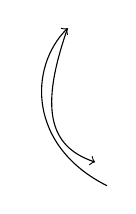
\begin{tikzpicture}[scale=.5]
\draw[->] (1,0) .. controls (-1,1) and (-1,3) .. (0,4);
\draw[->] (0,4) .. controls (-.7,2) and (-.5,1) .. (.7,.6);
\end{tikzpicture}}
\deleted{\diagram{\begin{array}{ccc}
\mathcal M_0&\unsure{\mathcal M_1}&\unsure{\mathcal M_N}\\
\downarrow&&\\
\unsure{P_k}&&
\end{array}}}
\deleted{\(\unsure{\operatorname{Hom}_k(P,Q)}\)}

\uline{Conditions équivalentes}

 a') \(\deleted{\unsure{\forall P\in\operatorname{Mod}k}}
 \operatorname{Imess}i\subset\operatorname{Imess}\rho_{0N}\)

 b') \(\forall P\in\operatorname{Mod}k,\quad
 iP\overset\sim\longrightarrow\rho_{0N}\tau_{N,0}\circ i(P)
 =\rho_{0N}i_N(P)\)

 \unsure{b') bis} \(\forall P\in\operatorname{Mod}k,\quad
 i(P)\overset\sim\longrightarrow\rho_{0N}i_N(P)\) est un isom en degrés
 \(0\leq\alpha\leq N-1\).

 c') \(\inserted{\forall P\in\operatorname{Mod}k,}\quad
 \forall\ 0\leq\alpha\leq N-1,\quad
 \deleted{\unsure{\tau_{N-\alpha,0}S\longrightarrow0}}\)
\diagram{\begin{tikzcd}
P\otimes_k S_\alpha\arrow[r,"\sim"]&
\operatorname{Hom}^\alpha(\tau_{N-\alpha}S,\deleted{\unsure{P}}P\otimes_kS)\\
\bigl[\operatorname{Hom}^\alpha(S,P\otimes_kS)\arrow[u,"\simeq"]
\arrow[ur,dashed,"\text{restriction}"']&\bigr]
\end{tikzcd}}
\[
\operatorname{Hom}^\alpha(S/\tau_{N-\alpha}S,P\otimes_kS)=0.
\]
\margin{251}
\scanpage{253}
\margin{252}
\deleted{
\(J\subset A\)

\(H^*(X,J)^{\unsure{*}}\) à p.d.
\[
A\{(X_i)_{i\in I},(\unsure{Y_i})_{i\in I}\}/
(\textstyle\sum X_i-\pi,\sum Y_i-\omega,\sum dX_i,\sum dY_i)
\]
\figure{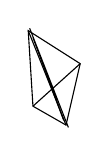
\begin{tikzpicture}[scale=.6]
\draw (0,2)--(.1,.4)--(.8,0)--(1.1,1.3)--cycle;
\draw (0,2)--(.8,0) (.1,.4)--(1.1,1.3);
\draw (.03,2.05)--(.85,-.05) (.1,1.85)--(.75,.1);
\end{tikzpicture}}
\[\deleted{A}\quad A^{(I)}\]
\[
\Gamma^*_{(A,\unsure{\pi|J})}(A^I\otimes_AJ)
\]
\[
\unsure{X_i|X_1}\otimes\pi,\ \unsure{X_2|X_i}\otimes\pi,\ -\ ,\ \unsure{X_n}\otimes\pi
\]
\[\sum X_i\otimes\pi-\pi\]
\deleted{\[J^I/J\]}
\[
\Gamma^*_{(A,\unsure{\omega|J})}(J^I)/\delta J
\]
\[
\delta\pi=\deleted{\unsure{\sum}}-\pi+\pi
\]
\[
C_A^*\qquad
A\{(X_i)_{i\in I}\inserted{,dX_i}\}/
\{\textstyle\sum\pi X_i-\pi,\pi\sum dX_i\}
\]
\[\Gamma_A^{*+}J\longrightarrow J\]
\[
H^*(X,\Gamma^{*+}J)\longrightarrow H^{\unsure{*|\alpha}}(X,J)
\]
\diagram{\begin{tikzcd}
&H^{\unsure{2\alpha|2i\alpha}}(X,\operatorname{Sym}^\alpha M)\\
H^{2i}(X,M)\arrow[r,"\gamma^\alpha"]&
H^{2i\alpha}(X,\Gamma^\alpha M)\arrow[u]
\end{tikzcd}}
\[
H^{2i}(X,J)\longrightarrow H^{2i\alpha}(X,\Gamma^\alpha J)
 \longrightarrow H^{2i\alpha}(X,J)
\]
\diagram{\begin{tikzcd}
A\arrow[r,no head,"2i"]\arrow[dr,"2i\alpha"']&M\\
&\Gamma^\alpha M
\end{tikzcd}}
\diagram{\begin{tikzcd}
\Gamma^i M\arrow[d,shift right]&x^{(i)}\arrow[d,mapsto]&
i!x^{(i)}=x^i\\
\operatorname{Sym}^i(M)\arrow[u,shift right]&x^i\arrow[ur,bend right]
\end{tikzcd}}
}
\scanpage{254}
\[
\mathcal M/\unsure{\mathrm{Neg}_\infty|\mathrm{Neg}_0}
 \simeq\varinjlim\mathcal M_N
\]
n'est pas une catégorie à \uline{lim} filtrantes exactes.
\margin{
\unsure{UNIVERSITE DES SCIENCES ET TECHNIQUES}\\
\unsure{DU LANGUEDOC}\\
\unsure{MATHEMATIQUES}\\
\unsure{Montpellier, le 16 Juin 1975}

\unsure{SEMINAIRE D'ANALYSE CONVEXE}

\unsure{Jeudi 19 juin 1975, à 11 h, Salle 431}

\unsure{Mr A. BENSOUSSAN - Professeur, Université Paris IX Dauphine.}

\unsure{Diffusions réfléchies.}
}
\margin{253}
\scanpage{255}
UNIVERSITE DES SCIENCES ET TECHNIQUES\\
DU LANGUEDOC

MATHEMATIQUES

Montpellier, le 16 Juin 1975

SEMINAIRE D'ANALYSE CONVEXE

Jeudi 19 juin 1975, à 11 h, Salle 431

Mr A. BENSOUSSAN - Professeur, Université Paris IX Dauphine.

Diffusions réfléchies.
\margin{\(\unsure{\mathcal M/\mathrm{Neg}_{\unsure{\infty|0}}\simeq\varinjlim\mathcal M_N}\)
\unsure{n'est pas une catégorie à lim filtrantes exactes.}}
\margin{254}
\scanpage{256}
\(S\)-module \(N\)-négligeable \(M\) \((N\in\mathbb Z)\)
\[
\overset{\mathrm{def}}\Longleftrightarrow\tau_NM=0
 \Longleftrightarrow M_i=0\text{ si }i\geq N
\]
module \(\infty\)-négligeable \(M\)
\[
\Longleftrightarrow\exists N\in\mathbb Z\text{ tel que }M\ \unsure{N\text{-négl.}}
\]
\[\Longleftrightarrow M_i=0\text{ si }i\text{ assez grand}\]
\uline{Remq} Si \(M\) de type fini, \(M\) est \(\infty\)-négligeable ssi
\(\exists N\geq0\) tel que \(\tau_NS\) annule \(M\).

\(M\) négligeable \(\Longleftrightarrow\) \(M\) limite inductive de modules
\(\infty\)-négligeables
\[
\Longleftrightarrow\text{tout sous-module de t.f. de }M\text{ est }\infty\text{-négligeable}
\]
\[
\Longleftrightarrow\forall x\in M,\quad\exists N\geq0\text{ tel que }\tau_NS\text{ annule }x
\]
\[
\mathrm{N\acute eg}_N\subset\mathrm{N\acute eg}_{N'}\subset
\mathrm{N\acute eg}_\infty\subset\mathrm{N\acute eg}
\qquad(N\leq N')
\]
\(\mathrm{N\acute eg}_N,\ \mathrm{N\acute eg}_\infty\) sous-catégories épaisses
de \(\mathcal M\),
\diagram{\begin{tikzcd}
\mathcal M/\mathrm{N\acute eg}_N\arrow[r,"\simeq"]\arrow[d]&
\mathcal M_N\arrow[d,"\tau_{N',N}"]\\
\mathcal M/\mathrm{N\acute eg}_{N'}\arrow[r]&\mathcal M_{N'}
\end{tikzcd}}
\margin{255}
\scanpage{257}
\[
\varinjlim\unsure{\varphi_N|\rho_N}\tau_NP
 \longrightarrow\unsure{\varphi_\infty|\rho_\infty}\tau_\infty P
\]
bijectif?
\deleted{\(\operatorname{Hom}\)}
\[\Updownarrow\]
\(\forall M\) de prés fini (il suffit \(M=S[i]\))
\diagram{\begin{array}{ccc}
\operatorname{Hom}_{\mathcal M}(M,\varinjlim\unsure{\varphi_N|\rho_N}\tau_NP)
 &\unsure{-|\longrightarrow}&
\operatorname{Hom}_{\mathcal M}(M,\unsure{\varphi_\infty|\rho_\infty}\tau_\infty P)
 \quad\text{bij.}\\
\simeq&&\simeq\\
\varinjlim\operatorname{Hom}_{\mathcal M}(M,\unsure{\varphi_N|\rho_N}\tau_NP)
 &&\operatorname{Hom}_{\mathcal M_\infty}(\tau_\infty M,\tau_\infty P)\\
\simeq&&\simeq\\
\varinjlim\operatorname{Hom}_{\mathcal M_N}(\tau_NM,\tau_NP)
 &&\underset{\substack{M'\subset M\\M/M'\ \text{négl.}}}{\varinjlim}
 \operatorname{Hom}(M',P)\\
\simeq&&\nearrow\\
\varinjlim\operatorname{Hom}_{\mathcal M}(\tau_NM,P)&&
\end{array}}
dire que (pour \(M\) fixé) c'est un isom pour \(\forall P\), signifie que les deux
proobjets de \(\mathcal M\) formés; soit des \(\tau_NM\), soit des
\(M'\subset M\) tels que \(M/M'\) est négligeable, \deleted{sont} isom par
l'hom can., ou encore que, ces \unsure{ens} de sous-objets sont cofinaux,
i.e que tout \(M'\) contient un \(\tau_NM\)
\inserted{i.e \(M/M'\) est \(\infty\)-négligeable.}
Mais c'est le cas si \(M\) de \deleted{\unsure{p.f.}}\inserted{t.f.}
\deleted{\uline{Hyp} Tout idéal gradué \(J\) de \(S\), tq que \(S/J\) soit
négligeable \unsure{finie.|fini.}}
Donc
\[
\varinjlim\unsure{\varphi_N|\rho_N}\tau_NP
 \overset\sim\longrightarrow\unsure{\varphi_\infty|\rho_\infty}\tau_\infty P
\]
\margin{256}
\scanpage{258}
U N I V E R S I T E\\
DES SCIENCES ET TECHNIQUES\\
\uline{DU LANGUEDOC}\\
AMC/MD

Montpellier, le 24 juin 1975

\uline{Diffusion} : Liste A\\
n\textsuperscript{o} 4135

AVIS DE SOUTENANCE D'UNE THESE DE DOCTORAT DE

\uline{SPECIALITE : CHIMIE}

Mention Chimie Organique Physique

\uline{Nom et prénom du candidat} : DALVERNY Gilbert

\uline{Titre de la thèse} : Synthèse et réactivité d'organomagnésiens perfluorés.
Application à la préparation d'acides perfluorosulfoniques et carboxyliques.

\uline{Date, heure et lieu de soutenance prévus} : 10 juillet 1975 à 11 heures, salle
de cours n\textsuperscript{o} 9 - U.S.T.L.

\uline{Nom du Directeur de thèse} : Monsieur le Professeur A. COMMEYRAS

\uline{Désignation du laboratoire où la thèse est préparée} : Laboratoire de chimie organique

\uline{Analyse de l'ouvrage} : Des méthodes de synthèses, par voie chimique, d'acides
perfluoroalcanesulfoniques \(\mathrm{R_FSO_3H}\) et carboxyliques \(\mathrm{R_FCO_2H}\)
ont été mises au point ; elles font intervenir comme intermédiaires réactionnels, les
organomagnésiens perfluorés saturés \(\mathrm{R_FMgX}\) correspondants.\\
Des possibilités d'application de la réaction magnésienne au niveau de composés
perfluorés insaturés ont été ensuite étudiées.

\uline{Durée approximative des recherches ayant abouti à la thèse} : 2 ans

\uline{Composition du jury proposé} : M. A. COMMEYRAS - Président\\
M. R. CORRIU\\
M. A. CAMBON\\
M. R. MARTIN

Le Secrétaire Général,
\figure{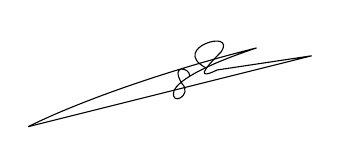
\begin{tikzpicture}[x=1cm,y=1cm]
\draw (0,0) .. controls (.6,.3) and (1.7,.7) .. (2.9,1)
 .. controls (2.3,.8) and (1.9,.6) .. (1.85,.45)
 .. controls (1.8,.25) and (2.1,.4) .. (1.95,.55)
 .. controls (1.8,.8) and (2.05,.75) .. (2.05,.65);
\draw (2.25,.75) .. controls (1.8,1) and (2.65,1.25) .. (2.45,.95)
 .. controls (2.2,.7) and (2.15,.6) .. (2.4,.72)
 --(3.6,.9)--(0,0);
\end{tikzpicture}}
\uline{E. SIAU}
\margin{257}
\scanpage{259}
\[
\begin{aligned}
(\varphi_\infty\tau_\infty P)_i
 &\simeq\operatorname{Hom}^i(S,\varphi_\infty\tau_\infty P)\\
 &\simeq\operatorname{Hom}(S[-i],\varphi_\infty\tau_\infty P)\\
 &\simeq\operatorname{Hom}(\tau_\infty S[-i],\tau_\infty P)\\
 &\simeq\underset{\substack{M'\subset S[-i]\\
 \text{t.q. }S[\unsure{-i|i}]/M'\ \text{négl.}}}{\varinjlim}
 \operatorname{Hom}(M',P)\\
 &\simeq\underset{\substack{M'\subset S\\\text{t.q. }S/M'\ \text{négl}}}{\varinjlim}
 \operatorname{Hom}^i(M',P)\\
 &\simeq\varinjlim_N
 \underbrace{\operatorname{Hom}^i(\tau_NS,P)}_{
 \simeq\operatorname{Hom}^i(\tau_NS,\tau_{N+i}P)}\\
 &\simeq\varinjlim_N\operatorname{Hom}(\tau_N(S[-i]),\tau_NP).
\end{aligned}
\]
\uuline{\hspace{10em}}
\diagram{\begin{tikzcd}
\tau_NS\arrow[r,"\mathrm d^\circ0"]\arrow[d,"{\cdot T^{(\ell)}}"']&P\\
\tau_{N+\ell}(S)\arrow[ur,"{\mathrm d^\circ\unsure{-\ell|\ell}}"']&
\end{tikzcd}}
\[
\unsure{\zeta|\xi}T^{(i)}\overset{T^{(\ell)}}\longmapsto
 \zeta c_{i,\ell}T^{(i+\ell)}
\]
\[
P\in\operatorname{Imess}\varphi_\infty
\quad\Updownarrow\quad
P\overset\sim\longrightarrow\varphi_\infty\tau_\infty P
\quad\Updownarrow
\]
\[
\operatorname{Hom}^i(S,P)\overset\sim\longrightarrow
 \varinjlim_N\operatorname{Hom}^i(\tau_NS,P)
\]
a) \uline{injectivité} : \(P\) n'a pas d'élément négligeable non nul

b) surjectivité : tout homom. \inserted{(homog)} d'un
\deleted{\unsure{idéal}} \(\tau_NS\) dans \(P\) se prolonge à \(S\), ou encore:
toute ext. de \([S/\tau_NS][-i]\) par \(P\) est triviale ....
\figure{\begin{tikzpicture}[scale=.5]
\draw[->] (0,0)--(4,4)--(1.5,7);
\end{tikzpicture}}
\margin{258}
\scanpage{260}
- \mspage{99} - \margin{IX}

que l'on a une \uline{immersion ouverte} canonique
\[
(8.3.1)\qquad A_{K,K'}^{\unsure{\natural|\sharp}}
 \hookrightarrow A_{K,K''}^{\unsure{\natural|\sharp}},
\]
permettant d'identifier le premier groupe à un sous-groupe ouvert du deuxième.
Pour \(K'\) variable, on voit que les \(A_{K,K'}\) forment ainsi un système inductif
de groupes lisses de type fini sur \(K\), à morphismes de transition des immersions
ouvertes. Si on pose
\[
(8.3.2)\qquad\Phi_{K,K'}=
 A_{K,K'}^{\unsure{\natural|\sharp}}/A_{K,K'}^{\unsure{\natural|\sharp}\,0},
\]
les \(\Phi_{K,K'}\) eux-mêmes forment donc un système inductif de groupes finis
étales sur \(K\), qui sera étudié plus en détail plus bas.

Nous poserons
\[
(8.3.3)\qquad A_K^{\unsure{b|\flat}}=
 \varinjlim_{K'}A_{K,K'}^{\unsure{\natural|\sharp}},
\]
la limite étant prise dans la catégorie des faisceaux fppf sur \(K\). Comme
les morphismes de transition dans le système inductif envisagé dans des immersions
ouvertes, il est d'ailleurs clair que cette limite est en fait représentable
par un schéma en groupes (en général non quasi-compact) sur \(K\), que nous
désignerons comme de juste par le même symbole \(A_K^{\unsure{b|\flat}}\).
On notera qu'on a, pour ce schéma en groupes
\margin{\figure{\begin{tikzpicture}[scale=.3]
\draw[line width=1pt] (0,0)--(.8,0);\draw (.1,.3)--(.3,.35)--(.4,.3);
\end{tikzpicture}}}
\[
(8.3.4)\qquad A_K^{\unsure{b|\flat}\,0}=A_K^{\unsure{\natural|\sharp}\,0},\quad
 A_K^{\unsure{b|\flat}}/A_K^{\unsure{b|\flat}\,0}
 \simeq\varinjlim_{K'}\Phi_{K,K'}.
\]
Ce dernier groupe sera déterminé dans 11.10 : il est canoniquement isomorphe
à \(\underline M_K\otimes\mathbb Q/\mathbb Z\) (avec la notation (8.1.8)).
\margin{417}
\margin{417}
\margin{259}
\scanpage{261}
\[
\operatorname{Hom}_{\mathcal M}(M,\varphi_N\deleted{\tau_N}
 \underset{\mathcal M_N\ \uparrow}{P})
 \simeq\operatorname{Hom}_{\mathcal M_N}(\tau_NM,\deleted{\tau_N}P)
\]
donc
\[
\begin{aligned}
(\varphi_N\tau_NP)_i
 &=\operatorname{Hom}^i_{\mathcal M}(S,\varphi_N\tau_NP)
 =\operatorname{Hom}_{\mathcal M}(S[-i],\varphi_N\deleted{\tau_N}P)\\
 &=\operatorname{Hom}_{\mathcal M_N}(\tau_N(S[-i]),\deleted{\tau_N}P)\\
 &\simeq\operatorname{Hom}_{\mathcal M_N}((\tau_{N-i}(S))(-i),\deleted{\tau_N}P)\\
 &\simeq\operatorname{Hom}^i_{\mathcal M}(\tau_{N-i}(S),\deleted{\tau_N}P).
\end{aligned}
\]
\uline{\hspace{15em}}
\(h_M=\operatorname{Hom}(M,-)\), donc
\[
h_M\circ\varphi_N\circ\deleted{\tau_N}\simeq
 h_{\tau_NM}\deleted{\circ\tau_N}
\]
\deleted{donc \(h_M\circ\varphi_N\circ\tau_N\simeq h_{\tau_NM}\circ\tau_N\)}
\deleted{\[\mathrm R^*(h_M\circ\varphi_N\tau_N)\simeq\mathrm R^*h_{\unsure{\tau}}\]}
Composons avec \(\tau_N\), on a
\[
\begin{aligned}
\operatorname{Hom}_{\mathcal M}(M,\varphi_N\tau_NP)
 &=\operatorname{Hom}_{\mathcal M_N}(\tau_NM,\tau_NP)\\
 &\simeq\operatorname{Hom}_{\mathcal M}(i_N\tau_NM,P).
\end{aligned}
\]
\[h_M\varphi_N\tau_N=h_{i_N\tau_N}\]
D'où
\diagram{\begin{array}{ccc}
\mathrm R^*(h_M\varphi_N\tau_N)&\simeq\mathrm R^*h_{i_N\tau_N}
 &=\mathrm R\operatorname{Hom}(i_N\tau_NM,-)\\
\Vert&&\\
\deleted{\unsure{\mathrm R}}\mathrm R^*(h_M\varphi_N)
 \underbrace{\tau_N}_{\mathrm R^*\tau_N\ \text{car }\tau_N\text{ exact}}&&
\end{array}}
Si \(M\) \uline{projectif} donc \(h_M\) exact, on aura
\[
h_M(\mathrm R^*\varphi_N)\circ\tau_N\simeq
 \mathrm R\operatorname{Hom}(\tau_NM,-)
\]
i.e.
\[
\boxed{\deleted{\unsure{\mathrm R}}\uline{\operatorname{Hom}}(M,\mathrm R^*\varphi_N(\tau_NP))
 \simeq\mathrm R\operatorname{Hom}(\tau_NM,P)}
\]
en particulier:
\deleted{\(\operatorname{Ext}\)}
\[
\boxed{\begin{gathered}
\operatorname{Hom}(M,(\mathrm R^n\varphi_N)(\tau_NP))
 =\operatorname{Ext}^n(\tau_NM,P)\\
\text{si }M\text{ projectif }\in\mathcal M
\end{gathered}}
\]
\margin{260}
\scanpage{262}
- \mspage{94} - \margin{IX}

la biextension \(W^{\mathrm{ab}}\) de \((B,B')\) par \(\mathbb G_{mS}\) est une
dualité parfaite sur \(U\) (ou ce qui revient au même si \(U\) est dense dans
\(S\), sur \(\unsure{S}\)). C'est une propriété qu'il suffit de vérifier en tout
point \(\eta\) de \(\unsure{U}\), et alors l'argument habituel nous ramène au cas où
\(S\) est un \unsure{trait} de point générique \(\eta\), qui est déjà connu.

La relation d'orthogonalité nous permet d'autre part d'étendre au cas présent
les formules (5.5.7), (5.5.8) et (5.5.9), où on remplace l'opération de restriction
au point générique \(\eta\) par celle de restriction à l'ouvert \(U\) ; par suite,
5.6 s'étend également au cas présent. Nous nous dispensons de réécrire ici les
formules et l'énoncé précédents dans le contexte présent.

Résumons, du point de vue des modèles de Néron, les résultats obtenus concernant
les parties abéliennes et leurs accouplements :

\uline{Proposition} 7.5. \uline{Soit} \(S\) \uline{un trait complet},
\uline{de corps de fonctions} \(K\). A \uline{tout schéma abélien} \(A_K\)
\uline{sur} \(K\) \uline{ayant une réduction semi-stable sur} \(S\),
\uline{le procédé de} 7.1,\uline{appliqué à la composante neutre du modèle de Néron}
\(A\), \uline{de} \(A_K\) \uline{permet de définir la} partie abélienne
\(B=A^{\mathrm{ab}}\) \uline{de celui-ci}, \uline{qui}
\uline{est un schéma abélien sur} \(S\), \uline{dépendant fonctoriellement de}
\(A_K\). \uline{Pour} \uline{tout autre schéma abélien} \(A'_K\)
\uline{à réduction semi-stable}, \uline{on peut à toute}
\uline{correspondance divisorielle} \(W_K\) \uline{sur} \((A_K,A'_K)\),
\uline{associer une correspondance} \uline{divisorielle unique} \(W^{\mathrm{ab}}\)
\uline{sur} \((A^{\mathrm{ab}},A'^{\mathrm{ab}})\),
\uline{telle que pour tout entier} \(n\geq0\), \(W_n^{\mathrm{ab}}\)
\uline{ait comme image inverse par}
\(A_n^0\longrightarrow B_n=A_n^{0\mathrm{ab}}\),
\(A'^0_n\longrightarrow B'_n=A'_n{}^{0\mathrm{ab}}\)
\uline{la biextension} \(W_n\) \uline{de} \((A_n^0,A'^0_n)\)
\uline{déduite de} \(W\) \uline{par} \uline{réduction}, \uline{où} \(W\)
\uline{est le prolongement canonique} (1.4) \uline{de} \(W_K\) \uline{à}
\((A^0,A'^0)\).
\margin{\figure{\begin{tikzpicture}[scale=.3]
\draw (0,.4)--(.2,.4);\fill (.15,0) circle (.035);\fill (.3,-.06) circle (.035);
\end{tikzpicture}}}
\margin{412}
\margin{412}
\margin{261}
\scanpage{263}
\uline{Ex} \(M=S[-i]\), on a
\[
\begin{aligned}
\kappa_i(\mathrm R^*\varphi_N(\tau_N(P)))
 &\simeq\mathrm R\operatorname{Hom}(\tau_N(S[-i]),P)\\
 &\simeq\mathrm R\operatorname{Hom}((\tau_{N-i}S)[-i],P)\\
 &\simeq\mathrm R\operatorname{Hom}^i(\tau_{N-i}S,P).
\end{aligned}
\]
donc
\[
(\mathrm R^n\varphi_N(\tau_NP))_i
 =\operatorname{Ext}^n((\tau_{N-i}S)[-i],P)
\]
\uline{NB} C'est valable aussi en remplaçant \(\varphi_N\) par
\(\varphi_{N',N}\) \((N'\leq N)\) pourvu que \(i\geq N'\)
(si \(i<N'\), on trouve \(0\) bien sûr!)
\deleted{
\uline{NB} Supposons \(P\in\operatorname{Imess}\varphi_{N',N}\) \((N'\leq N)\)
i.e \(\deleted{\unsure{\varphi_N}}P\overset\sim\longrightarrow
\varphi_{N',N}\tau_NP=\mathrm R^0\varphi_{N',N}(\tau_NP)\)
Alors
\[
\mathrm R^n(\varphi_{N',N}(\tau_NP))=0\text{ si }n>0
\]
i.e
\[
\operatorname{Ext}^n(\tau_{N-i}(S)[-i],P)=0
 \text{ si }\begin{cases}i\geq N'\\n>0\end{cases}
\]
En effet, cela revient à
\[\unsure{\mathrm R^n\varphi_N\tau_N(Q)}\quad
 \underset{\mathcal M_N\ \uparrow}{Q}\]
}
\margin{\(\unsure{N'_0|N_0}\leq N\text{ dans }\mathbb Z\)}
Soit \(C\) une catégorie abélienne, et
\[C\overset{i}\longrightarrow\mathcal M_{N'_0}\]
un foncteur \uline{exact}, tel que
\[i(C)\subset\operatorname{Imess}\varphi_{N'_0,N}\]
i.e
\[
i(M)\overset\sim\longrightarrow\varphi_{N'_0,N}\tau_{N,N'_0}i(M)
\]
je dis qu'alors
\[
(\mathrm R^n\varphi_{N'_0,N})(\tau_{N,N'_0}\circ i)=0
 \quad\text{si }n>0
\]
En effet, comme \(i\simeq\varphi_{N'_0,N}\tau_{N,N'_0}i\)
on conclut
\diagram{\begin{array}{ccc}
\mathrm R^*i&\simeq&\mathrm R^*(\unsure{\varphi_{N'_0,N}\tau_{N,N'_0}\circ i})\\
\simeq&&\simeq\\
i&&(\mathrm R^*\varphi_{N'_0,N})(\tau_{N,N'_0}\circ i)
\end{array}}
\margin{car \(i\) exact}
\margin{car \(\unsure{\tau_{N,N'_0}\circ i}\) exact}
\margin{262}
\scanpage{264}
- \mspage{76} - \margin{IX}

de prolonger ce groupe de Barsotti-Tate en un sous-groupe de Barsotti-Tate
\(F\) de \(A\), qui jouerait alors le rôle joué par la \uline{partie fixe}
\(T_\ell(A)^{\mathrm f}\) de (2,2.3.2) dans le cas où \(A^0\) est
\(\ell\)-divisible. Dans le cas semi-stable, où on a \(\overline A_0=A_0^0\),la
question se résoud par l'affirmative par la méthode de 2.2. Dans le cas général,
lorsque le problème envisagé a une solution, on voit facilement qu'elle est
unique, et que les sous-pro-groupes correspondants de \(T_p(A_K)\) et de
\(T_p(A'_K)\) (qui méritent alors encore le nom de \uline{partie fixe} des
pro-groupes envisagés) satisfont encore au théorème d'orthogonalité 5.2, enfin que
la partie fixe \(T_p(A_K)^{\mathrm f}\) peut encore se caractériser comme indiqué
dans 5.3.

6.2.1. Montrons cependant qu'en général le problème envisagé n'a pas une
solution affirmative, i.e. qu'\uline{il n'est pas possible en général de}
\uline{définir la partie fixe} \(T_p(A)^{\mathrm f}\) (cas de la réduction non
semi-stable). En effet, en vertu d'un théorème de relèvement de SERRE-TATE [30],
lorsque \(S\) est complet, l'existence de la partie fixe équivaut à celle de
relèvements infinitésimaux \(\overline A_n\) de \(\overline A_0\) dans les
\(A_n\), ou encore à celle d'un schéma en groupes lisse \(\overline A\) sur
\(S\), extension d'un schéma abélien par un tore \(T\), de fibre spéciale
\(\overline A_0\), et d'un homomorphisme formel
\(\widehat{\overline A}\longrightarrow\unsure{\widehat A|A}\) prolongeant
l'inclusion sur les fibres spéciales. Donc, dans le cas où \(\overline A_0\)
est un schéma abélien i.e. où \(T_0=0\), cela équivaut à l'existence d'un schéma
abélien \(\overline A\) prolongeant \(\overline A_0\) et d'un homomorphisme
\(\overline A\longrightarrow A\) prolongeant l'inclusion des fibres spéciales.
Il suffira donc de donner un cas où \(T_0=0\), où \(A_0^0\) est non unipotent
et non propre, et où \(A_K\) est simple sur \(K\).
\margin{\figure{\begin{tikzpicture}[scale=.3]
\draw (0,.7)--(.3,.8)--(.15,.65);\draw (.7,.2)--(.9,.1);
\draw (1.4,0)--(1.55,.05);
\end{tikzpicture}}}
\margin{394}
\margin{394}
\margin{263}
\scanpage{265}
d'où la conclusion

Le cas qui nous intéresse est
\[
N'_0=0\leq N,\quad C=\operatorname{Mod}(k),
\]
\(i(M)=M\otimes_k S,\) et si on sait que
\[
M\otimes_k S\subset\operatorname{Imess}\varphi_{0N}\qquad\forall M\in\operatorname{Mod}(k)
\]
i.e.
\[
M\otimes_k S\simeq\varphi_{0N}\tau_N(M\otimes_k S)
\bigl(=R^0\varphi_{0N}(\unsure{\tau_N M\otimes_k S})\bigr)
\]
\[
\deleted{\unsure{\Vert}\quad\operatorname{Hom}((\tau_{N-i}S)[-i],M\otimes_{\unsure{k}})}
\]
alors on a
\[
R^n\varphi_{0N}(\tau_N(M\otimes_k S))=0\quad\text{si }n>0
\]
i.e.
\[
\boxed{\operatorname{Ext}^n_{\mathcal M}((\tau_{N-i}S)[-i],M\otimes_k S)=0\quad\text{si }n>0,\ i\geq0}
\]
\figure{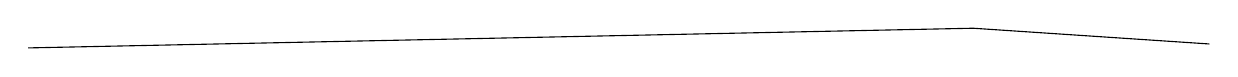
\begin{tikzpicture}\draw (0,0)--(12,.25)--(15,.05);\end{tikzpicture}}
\[
\operatorname{Hom}_{\mathcal M}(M,\varphi_\infty\tau_\infty P)\simeq\ldots
\underset{\text{si }M\text{ de prés. finie}}{\simeq}
\varinjlim_N\operatorname{Hom}_{\mathcal M}^{\deleted{\unsure{*}}}(\tau_{N\deleted{\unsure{-i}}}M,\deleted{\unsure{\tau}}P)
\]
Si de plus \(M\) projectif
\[
\operatorname{Hom}(M,R^*\varphi_\infty(\tau_\infty P))\simeq
\varinjlim_N R\operatorname{Hom}_{\mathcal M}((\tau_{N\deleted{\unsure{-i}}}M)\deleted{\unsure{[-i]}},-)
\]
en particulier
\[
\operatorname{Hom}(M,R^n\varphi_\infty P)\simeq
\varinjlim_N\operatorname{Ext}_{\mathcal M}^n((\tau_{N-i}M)[-i],P)
\]
p.ex. si \(M=S[i],\) on trouve
\[
\deleted{R^*}(\varphi_\infty\tau_\infty P)_i=
\varinjlim_N\operatorname{Hom}^i(\tau_{N-i}S,P)
\]
\[
(R^*\varphi_\infty(\tau_\infty P))_{\unsure{i|0}}\simeq
\varinjlim_N R^*\operatorname{Hom}^i(\tau_{N-i}(S),P)
\]
\[
\deleted{\unsure{R\operatorname{Hom}^i}}
(R^n\varphi_\infty(\tau_\infty P))_i\simeq
\varinjlim_N\operatorname{Ext}_{\mathcal M}^n(\tau_{N-i}(S)[-i],P).
\]
\margin{264}
\scanpage{266}
- \mspage{84} -
\margin{IX}
\uline{Proposition} 7.1.5. \uline{Avec les notations précédentes pour} \(S,A,\hat B,\) \uline{supposons que} \(S\) \uline{soit} normal. \uline{Alors} \(\hat B\) \uline{est algébrisable, et le schéma abélien} \(B\) \uline{sur} \(S\) \uline{dont il provient est projectif sur} \(S.\)

On peut évidemment supposer \(A=A^0,\) et \(S\) intègre. D'après M. RAYNAUD [23 XI 1.13], l'hypothèse que \(S\) est normal implique que \(A\) est quasi-projectif sur \(S.\) Soit donc \(\uline{L}\) un Module inversible sur \(A\) qui est relativement ample, et formons le Module birigidifié
\(\delta(\uline{L})=\pi^*(\uline{L})\operatorname{pr}_1^*(\uline{L})^{-1}\operatorname{pr}_2^*(\uline{L})^{-1}\)
sur \(A\times_S A\) comme dans VIII 4.12. Comme les fibres de \(A_0\) sont de rang unipotent nul, il en est de même de celles de \(A\) (résulte facilement de 3.1), donc en vertu de VIII 7.5, \(\delta(\uline{L})\) définit une biextension \(W\) de \((A,A),\) évidemment symétrique, qui en vertu de VIII 4.13 (i.e. essentiellement en vertu de RAYNAUD [23 XI 1.11]) satisfait à la condition d'amplitude voulue en les points de \(S_0.\)

\uline{Remarque} 7.1.6. On peut prouver, sans hypothèse de normalité sur \(S,\) que \(\hat B\) est toujours algébrisable, en se ramenant au cas normal comme dans 13.5.3 a).

7.2. Notons maintenant le

\uline{Lemme} 7.2.1. \uline{Soient} \(S\) \uline{le spectre d'un anneau noethérien} \(V,\) \uline{séparé et complet pour la topologie définie par un idéal} \(\uline{m}\) \uline{de} \(V,\) \(C\) \uline{la catégorie des schémas en groupes} \(A\) \uline{sur} \(S,\) \uline{lisses de type fini sur} \(S,\) \uline{tels que} \(A/A^0\) \uline{soit un schéma en groupes étale fini sur} \(S\) \uline{et que} \(A^0\) \uline{soit une extension d'un schéma abélien} \(B\) \uline{par un tore isotrivial} \(T\) (SGA 3 IX 1.1),
\margin{402}
\margin{265}
\margin{402}
\scanpage{267}
Si \(\deleted{\unsure{C}}\ C\xrightarrow{i}\mathcal M_{N_0}\) est un foncteur exact
\[
\operatorname{Im}\deleted{\unsure{ess}}i\subset\operatorname{Imess}\varphi_{N_0,\infty}
\]
alors on a \(i\simeq\varphi_{N_0,\infty}\tau_{\infty,N_0}i\) d'où
\[
(R^*\varphi_{N_0,\infty})(\tau_{\infty,N_0}\circ i)\simeq R^*i
\]
en particulier
\[
(R^n\varphi_{N_0,\infty})(\tau_{\infty,N_0}i(M))=0\quad\text{si }n>0,\ M\in\operatorname{ob}C.
\]
On est intéressé aux mêmes cas particuliers qu'avant.
\figure{\begin{tikzpicture}\draw (0,0)--(1.4,0);\end{tikzpicture}}
Soit \(K^\bullet\) un complexe de \(C\)

\(L^\bullet\) un complexe de \(\mathcal M_{\deleted{\unsure{\infty}}}\)

et supposons donné un hom dans la catégorie dérivée \(D(\mathcal M_{N_0})\)
\[
i(K^\bullet)\xrightarrow{\alpha}L^\bullet
\]
tel que
\[
\tau_{\infty,N_0}i(K)\xrightarrow[\sim]{\tau_\infty\alpha}\tau_{\infty,N_0}L^\bullet
\]
soit un isom dans \(D(\mathcal M_\infty),\) i.e.

tel que \(\forall n,\)
\diagram{\begin{array}{ccc}
H^n(\alpha):&H^n(i(K))&\longrightarrow H^n(L^\bullet)\\
&\rotatebox{90}{\(\simeq\)}&\\
&i(H^n(K))&
\end{array}}
soit un \(\infty\)-isom i.e. noyau et conoyau sont négligeables. On en conclut
\margin{266}
\scanpage{268}
\margin{\figure{\begin{tikzpicture}\draw[<-] (0,0)--(.5,0);\end{tikzpicture}}}
- \mspage{83} -
\margin{IX}
7.1.3. La projectivité de \(\hat B\) signifie, en vertu de EGA III 5.4.5, que l'on peut trouver un Module inversible \(\hat{\uline{M}}\) sur \(\hat B,\) i.e. une suite de Modules inversibles \(\uline{M}_n\) sur les \(B_n\) qui se ``\unsure{recollent}'' pour \(n\) variable, qui soit \uline{ample} relativement à \(S\) i.e. qui soit tel que \(M_0\) soit ample. L'idée naturelle serait de partir d'un Module inversible ample \(\uline{M}\) de \(G,\) et de montrer que pour tout \(n,\) la restriction \(\uline{L}_n\) de \(\uline{L}\) à \(G_n\) provient par image inverse d'un Module inversible \(M_n\) sur \(B_n.\) J'ignore si de tels \(M_n\) existent nécessairement (et en doute fort). Nous allons suivre une méthode un peu différente, en construisant une \uline{polarisation} de \(B,\) i.e. un système projectif de \uline{polarisations} \(\rho_n\) des \(B_n\) qui se recollent. On sait alors [5] que les doubles de ces polarisations définissent canoniquement des Modules inversibles \(\uline{M}_n\) (symétriques) sur les \(B_n,\) qui par leur nature canonique se recolleront nécessairement, et fourniront le \(\unsure{\hat{\uline{M}}|\uline{M}}\) cherché.

Nous allons interpréter un élément de \(\operatorname{NS}(B_n/S_n)\) comme une correspondance divisorielle symétrique sur \((B_n,B_n)\) [5], i.e. comme une biextension de \((B_n,B_n)\) par \(\mathbb G_{m\,S_n}.\) En vertu de VIII 3.5, ces biextensions correspondent biunivoquement aux biextensions de \((A_n,A_n)\) par \(\mathbb G_{mS}.\) Pour obtenir un système cohérent de telles biextensions \(W_n\) il suffit de partir d'une
\[
(7.1.4)\qquad W,\ \text{biextension symétrique de }(A,A)\text{ par }\mathbb G_{mS},
\]
en prenant les \(W_n\) se déduisant de \(W\) par les changements de base \(S_n\longrightarrow S.\) Nous devons de plus supposer que l'élément de \(\operatorname{NS}(B_0)\) défini par \(W_0\) est une polarisation de \(B_0\) pour obtenir ainsi une polarisation de \(\hat B.\)
\figure{
\begin{tikzpicture}\fill (0,0)--(.06,.10)--(.12,.02)--(.20,.13)--(.16,-.03)--(.06,-.04)--cycle;\end{tikzpicture}}
\margin{401}
\margin{267}
\margin{401}
\scanpage{269}
en appliquant \(R\varphi_{\unsure{0|\infty},\infty}\)
\[
\underbrace{(R^*\varphi_{N_0,\infty})(\tau_{\infty,\deleted{\unsure{i}}N_0}i)(K)}
\simeq(R^*\varphi_{N_0,\infty})(\tau_{\infty,N_0}L^\bullet)
\]
i.e.
\[
i(K)\simeq\underbrace{(R^*\varphi_{N_0,\infty})(\tau_{\infty,N_0}L^\bullet)}_{\unsure{L'^\bullet|L'}}
\]
\deleted{Je dis que l'hom d'augmentation \(L^\bullet\to\)}

Mais c'est là un isom dans \(D(\mathcal M_{N_0})\) seulement -- rien de plus précis que la donnée de départ -- on aimerait un isom dans \(D(C).\) On va supposer \(i\) pl. fidèle et avec un adjoint à droite \(\kappa,\) donc
\[
\kappa\circ i\simeq\operatorname{id}_C
\]
et on va supposer \(\kappa\) \uline{exact}: Appliquons \(\kappa\) à l'isom obtenu on trouve
\[
K^\bullet\simeq\kappa\bigl(R^*\varphi_{N_0,\infty}(\tau_{\infty,N_0}L^\bullet)\bigr)
\inserted{\simeq(R^*(\kappa\varphi_{N_0,\infty}))(\tau_{\infty,N_0}L^\bullet)}
\]
i.e. \(K^\bullet\) se reconstruit dans \(D(C)\) à l'aide de \(\tau_{\infty,N_0}(i(K^\bullet))\) \deleted{\unsure{donc}} \(\tau_{\infty,N_0}(L^\bullet)\) dans \(D(\mathcal M_\infty).\)
\deleted{On va simplifier l'expression obtenue, en considérant
\[
\varphi_{N_0,\infty}(\tau_{\infty,N_0}(L^\bullet))\longrightarrow
R^*\varphi_{N_0,\infty}(\tau_{\infty,N_0}L^\bullet)
\]
\uline{Lemme} Cet hom est un quasi-isomorphisme

\uuline{Corollaire}
\[
K^\bullet\simeq\kappa\varphi_{N_0,\infty}(\tau_{\infty,N_0}L^\bullet)
\simeq\kappa\varphi_{N_0,\infty}(\tau_{\infty,N_0}iK).
\]}
\margin{268}
\scanpage{270}
- \mspage{82} -
\margin{IX}
par un tore. Nous avons posé comme d'habitude \(A_n=A\times_S S_n,\) où \(S_n=\operatorname{Spec}(V/\uline{m}^{n+1}).\) Nous nous intéresserons surtout au cas où \(S\) est un trait, et où la fibre générique \(A_K\) est un schéma abélien à réduction semi-stable sur \(S,\) \(A\) étant le modèle de Néron de \(A_K.\)

Soit \(T_0\) le tore maximal de \(A_0,\) de sorte que \(B_0=A_0^0/T_0\) est un schéma abélien. La construction de 5.1 s'applique alors pour fournir un sous-tore formel \(\hat T\) du complété formel \(\hat A.\) On sait que pour tout \(n,\) le quotient
\[
(7.1.1)\qquad B_n=A_n^0/T_n
\]
est représentable (SGA 3 VI\(_A\) 3.2), plus précisément c'est un schéma plat et de type fini sur \(S_n,\) dont l'image inverse sur \(S_0\) est le schéma abélien \(B_0.\) Par suite \(B_n\) est un \uline{schéma abélien} sur \(S_n,\) et pour \(n\) variable, les \(B_n\) se déduisent les uns des autres par changement de base, donc ils définissent un \uline{schéma abélien formel}
\[
(7.1.2)\qquad\hat B=(B_n)_{n\geq0}.
\]
Nous allons donner des conditions impliquant que ce schéma abélien est \uline{algébrisable} (EGA III 5.4.1), plus précisément que c'est le complété formel d'un schéma abélien projectif sur \(S,\) que nous noterons alors \(B.\) En vertu de loc.cit. \(B\) est déterminé à isomorphisme unique près (comme \(S\)-schéma ; la structure de groupe de \(\hat B\) provient alors de façon unique d'une structure de groupe de \(B,\) en vertu de loc. cit. également). Ce schéma abélien \(B\) sera alors appelé \uline{la partie abélienne} du schéma \(A,\) et parfois noté \(A^{\mathrm{ab}}.\)
\margin{400}
\margin{269}
\margin{400}
\scanpage{271}
\diagram{\begin{tikzcd}
C\arrow[r,"{\unsure{\tau_{\infty,N_0}|\varphi_{\infty,N_0}}i=\sigma}"']&\mathcal M_\infty\arrow[l,bend left=65,"{\kappa\varphi_{N_0,\infty}=\psi}"']
\end{tikzcd}}
\(\sigma\) pl. fidèle, adj. à droite \(\psi\)
\[
\psi\sigma\xleftarrow{\sim}\operatorname{id}_C\qquad
\left|\begin{array}{l}\deleted{\psi\text{ exact}}\\\sigma\text{ exact}\\\kappa\text{ exact}\end{array}\right.
\]
mais \(\psi\) peut-être pas exact
\[
\deleted{\unsure{R}}\quad\sigma(K^\bullet)\longrightarrow L^\bullet_\infty\qquad\text{quasi-isom dans }\mathcal M_\infty
\]
\deleted{
\diagram{\begin{array}{ccc}
(R^*\psi)\underbrace{\sigma(K^\bullet)}_{\Vert\ R^*\sigma K}&\xrightarrow{\sim}R^*\psi(L^\bullet_\infty)&\xleftarrow{\overset{?}{\sim}}\psi(L^\bullet_\infty)\\
\Vert&&\\
R^*(\underbrace{\psi\sigma}_{\simeq\mathrm{id}})(K)\simeq K&&
\end{array}}
\diagram{\begin{tikzcd}
\begin{gathered}\deleted{\unsure{R^n\psi}}\\H^*(R\psi(L^\bullet_\infty))\end{gathered}&\\
E_2^{pq}=R^q\psi(H^p(L^\bullet_\infty))\arrow[u,Rightarrow]&
\end{tikzcd}}
Si \(R^q\psi(H^p(L^\bullet_\infty))=0\) pour \(q>0\)
\[
\deleted{E_1^{pq}\longrightarrow E_1^{p+1,q}}\qquad
\deleted{E_2^{pq}\longrightarrow E_2^{p+2,q-1}}
\]
On trouve
\[
H^n(R\psi(L^\bullet_\infty))\simeq\psi(H^n(L^\bullet_\infty))
\]
}
\deleted{
\[
i(K^\bullet)\longleftarrow L^\bullet
\]
\[
\tau_{\infty,N_0}i(K^\bullet)\xleftarrow{\sim}\tau_{\infty,N_0}(L^\bullet)
\]
\[
K^\bullet\simeq R^*(\kappa\circ\varphi_\infty)(\tau_{\infty,N_0}(L^\bullet))
\]
\[
D(\operatorname{Mod}(k))\xrightarrow{\text{pl. fidèle}}D(\mathcal M_\infty)
\]
}
\margin{270}
\scanpage{272}
- \mspage{81} -
\margin{IX}
opère (de façon non nécessairement fidèle) sur \(k'\) (le corps des invariants étant \(k\)), et sur \(Y_{k'}\) da façon compatible avec son action sur \(k'.\) Or, d'après la théorie de DIEUDONNÉ [16 bis], au \(p\)-pro-groupe de Barsotti-Tate \(Y_{k'}\) est canoniquement associé un module \(M\) libre de type fini (de rang égal au rang de \(Y_{k'}\)) sur l'anneau \(W(k')\) des vecteurs de Witt sur \(k',\) et \(G\) opère évidemment sur \(M\) de façon compatible avec ses opérations sur \(W(k')\) (via ses opérations sur \(k'\)). On en déduit une opération \(W(k')\)-linéaire du sous-groupe d'inertie \(\Gamma\) de \(G\) sur \(M\) (qui est un quotient du groupe d'inertie \(I\)), d'où une fonction trace sur \(\Gamma\) donc sur \(I,\) qui est la fonction cherchée.Elle est a priori à valeurs dans \(W(k')\) (*), mais coïncide avec la fonction analogue définie en termes des \(T_\ell\) pour \(\ell\neq p,\) lorsque l'opération de \(G\) sur \(Y_{S'}\) s'obtient à partir d'une opération de \(G\) sur un schéma en groupes lisse et \(p\)-divisible \(C'\) sur \(S',\) en prenant \(Y=T_p(C')\) (cf. [25 bis, th.7 p.737]) ; elle est donc dans ce cas à valeurs entières. On procède de façon analogue dans le cas de 4.3 b) pour définir une fonction trace sur \(\pi^!,\) en utilisant le procédé de la démonstration de 4.3.2 pour ``linéariser'' l'opération dans \(M\) définie par un élément \(g\in\pi\) qui se trouve au-dessus d'un \(f_q{}^n\) avec \(n\geq0.\)

7. \uline{L'extension de Raynaud} \(G^{\unsure{\natural|\sharp}}\) \uline{sur} \(S\) \uline{attachée au schéma abélien} \(A_K\) \uline{à réduction semi-stable}. \uline{Dualité des schémas abéliens} \(B,B'\) \uline{sur} \(S.\)

7.1. Soit \(S\) un schéma noethérien spectre d'un anneau \(V,\) séparé et complet pour la topologie définie par un idéal \(\uline{m}\) de \(V.\) Soit \(A\) un schéma en groupes lisse sur \(S,\) \(A^0\) sa composante neutre, et supposons que \(A_0/A_0^0\) soit fini (donc fini étale) sur \(S_0,\) et que \(A_0^0\) soit une extension d'un schéma abélien

\margin{(*) En fait, il est immédiat que cette fonction est toujours à valeurs dans \(W(k),\) étant invariante par \(\operatorname{Gal}(k'/k).\)}
\figure{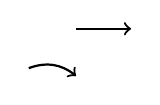
\begin{tikzpicture}\draw[->,thick] (0,0)--(.7,0);\draw[->,thick] (-.6,-.5) to[bend left] (0,-.6);\end{tikzpicture}}
\margin{399}
\margin{271}
\margin{399}
\scanpage{273}
\deleted{\(\psi\sigma=\operatorname{id}\)}
\diagram{\begin{tikzcd}
D^+(C)\arrow[r,"R\sigma"]&D^+(\mathcal M_\infty\arrow[l,bend left=50,"R\psi"']
\end{tikzcd}}
\margin{\(\psi\sigma\xleftarrow{\sim}\operatorname{id}_C\)\quad
\(\sigma\psi\longrightarrow\operatorname{id}_{\mathcal M_\infty}\)}
\diagram{\begin{tikzcd}[column sep=small]
&\operatorname{Hom}(R\sigma K,\underbrace{R\sigma R\psi(L)}_{R(\sigma\psi)(L)})\arrow[dl]&\\
\operatorname{Hom}(R\sigma(K),L)\arrow[rr,"{\overset{?}{\sim}}"]\arrow[dr]&&\operatorname{Hom}(K,R\psi(L))\arrow[ul]\\
&\operatorname{Hom}(\underbrace{R\psi R\sigma K}_{R(\psi\sigma)(K)\simeq K},R\psi L)\arrow[ur,phantom,"\simeq",sloped]&
\end{tikzcd}}
\diagram{\begin{array}{cc}
R\sigma R\psi R\sigma K,&R\sigma R\psi L\\
\downarrow&\downarrow\\
R\sigma K&L
\end{array}}
\[
D^+C\longrightarrow D^+\mathcal M_\infty
\]
pl. fid.

compatible avec multiplication
\margin{272}
\scanpage{274}
- \mspage{80} -
\margin{IX}
\margin{\figure{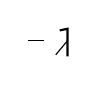
\begin{tikzpicture}\draw (0,0)--(.2,0);\draw[thick] (.5,-.2)--(.5,.15)--(.4,.13);\draw (.5,0)--(.35,-.18);\end{tikzpicture}}}
6.4. Notons que lorsque \(\ell\neq p,\) nous avons mis en évidence dans 4.3 a) une fonction à valeurs entières remarquable sur le groupe d'inertie \(I\) de \(S,\) d'ailleurs indépendante du choix de \(\ell,\) et dont la connaissance, dans le cas d'un corps résiduel parfait, suffit à reconstruire l'exposant conducteur de \(A\) (4.5), en prenant le produit scalaire, sur un quotient assez grand \(\Gamma=I/I'\) de \(I,\) de la fonction précédente et du conducteur d'Artin sur \(\Gamma\) (cf. (4.6.2)). Il peut être intéressant d'observer que cette fonction à valeurs entières sur \(I\) peut se réconstituer également par la connaissance de \(T_\ell(A_K)\) pour \(\ell=p\) - du moins (pour le moment) en inégales caractéristiques. Lorsque le corps résiduel \(k\) est fini, une observation analogue s'applique à la fonction à valeurs dans \(\mathbb Q,\) définie sur le sous-groupe \(\pi^!\) de \(\pi\) formé des éléments dont l'image dans \(\pi_0\) est de la forme \(f_q{}^n\) (\(n\in\mathbb Z\)), considérée dans 4.3 b). Indiquons le principe de la vérification de ces assertions. On utilise la filtration (6.3.1), et on est réduit à attacher une fonction convenable (sur \(I\) resp. sur \(\pi^!\)) à un \(p\)-pro-groupe de Barsoti-Tate \(Y\) sur \(K\) qui a ``essentiellement bonne réduction sur \(S\)'', au sens précisé dans 6.5. (\(Y\) sera un des trois quotients provenant de la filtration (6.3.1).) Dans le cas de 4.3 a), on se ramène au cas d'un corps résiduel parfait (ou même algébriquement clos, si on veut) par extension résiduelle convenable dans \(S\) (EGA 0\(_{\mathrm{III}}\) 10.3.1). Prenons alors une extension galoisienne finie \(K'\) de \(K\) telle que \(Y_{K'}\) ait bonne réduction sur \(S',\) d'où un groupe de Barsotti-Tate \(Y_{S'}\) sur \(S'\) et une opération de \(G\) sur \(Y_{S'}\) compatible avec son action sur \(S'.\) Si \(k'\) est le corps résiduel de \(S',\) \(G\)
\figure{\begin{tikzpicture}\draw[thick] (0,0) to[bend left=70] (.15,.1) to[bend left=70] (.25,0) to[bend left=70] (0,0);\draw (.9,0)--(.9,.2) (.8,.1)--(1,.1);\draw (2,0) to[bend left] (2.1,.2);\end{tikzpicture}}
\margin{398}
\margin{273}
\margin{398}
\scanpage{275}
\[
C\xrightarrow{i}\mathcal M\qquad M\longmapsto M\otimes_k S
\]
\[
i\xrightarrow{\sim}\varphi_{0,N}\tau_{N,0}\deleted{\unsure{\circ}}i\qquad0\leq i\leq N
\]
\diagram{\begin{array}{ccc}
&(x_k)_{k\geq N}\mathrel{\substack{\longrightarrow\\[-.4em]\longrightarrow}}&\unsure{c_{\ell,k}}x_k-c_{\ell,k-i}x_{k+\ell}\\
M\lhook\joinrel\longrightarrow&M^{[N,+\infty[}&\mathrel{\substack{\longrightarrow\\[-.4em]\longrightarrow}}M^{[N,+\infty]\times\mathbb N}\\
x\longmapsto&(c_{i,k-i}x)_{k\geq N}&
\end{array}}
\[
M\longmapsto\uline{\operatorname{Hom}}_k^*(S,M)
\]
\[
\varphi^{0,N}\tau^{N,0}\circ i\longrightarrow i
\qquad\text{syst. des }\uline{\operatorname{Hom}}_k(S_i,M)\simeq S\otimes_k M
\]
\(\operatorname{Ab}\qquad\operatorname{Ind}(\operatorname{Ab})\)
\[
M\otimes_k S_i\longrightarrow\uline{\operatorname{Hom}}^i(\tau_{N-i}(S),M\otimes_k S)
\]
\(C\) \unsure{Cat.} ab. \(k\)-linéaire (i.e. \(k\longrightarrow\operatorname{End}(\operatorname{id}_C)\))

\(X\) objet de \(C\)

\(M\) un \(k\)-module à g (resp à droite

\(\uline{\operatorname{Hom}}(M,X)\in C\) défini par
\[
\operatorname{Hom}(Y,\uline{\operatorname{Hom}}(M,X))=
\operatorname{Hom}_k(M,\operatorname{Hom}_C(Y,X))
\]
\(M\otimes_k X\) défini par
\[
\operatorname{Hom}(M\otimes_k X,Y)\simeq\operatorname{Hom}_k(M,\operatorname{Hom}_C(X,Y))
\]
Dans la mesure où ça existe
\[
M\longmapsto\uline{\operatorname{Hom}}(M,X)\quad\text{et}\quad M\longmapsto M\otimes_k X
\]
\unsure{est} exact à droite --
\margin{275}
\scanpage{276}
- \mspage{127} -
\margin{IX}
10.5. \uline{Réduction de} 10.4 \uline{à un cas particulier}.

10.5.1. L'unicité d'un \(u\) satisfaisant la condition énoncée (même pour un seul \(\ell\)) est claire. D'autre part, l'existence signifie simplement que chaque \(u_\ell\) applique en fait \(\uline{M}\otimes\uline{M}'\) dans \(\unsure{\mathbb Z_S}\) et que l'homomorphisme ainsi obtenu \(\uline{M}\otimes\uline{M}'\longrightarrow\mathbb Z_S\) est indépendant de \(\ell.\) En fait, il suffit même de prouver l'assertion analogue pour les \(u_\ell\otimes_{\mathbb Z_\ell}\mathbb Q_\ell\) et un \(u_{\mathbb Q}:\uline{M}_{\mathbb Q}\otimes\uline{M}'_{\mathbb Q}\longrightarrow\mathbb Q_S.\)

Supposons alors qu'on ait établi l'existence après changement de base \(S'\longrightarrow S\) comme dans 9.3. Alors il résulte immédiatement de (10.3.5) qu'il existe un homomorphisme
\[
u:\uline{M}\otimes\uline{M}'\longrightarrow\frac{1}{e(S'/S)}\mathbb Z_S\subset\mathbb Q_S
\]
compatible avec les \(u_\ell\otimes_{\mathbb Z_\ell}\mathbb Q_\ell,\) d'où a). Quant à b), il est trivial alors que s'il est vrai pour \(A_{K'},\) il l'est aussi pour \(A_K.\)

Par suite, nous pouvons, pour prouver 10.4, nous permettre n'importe quel changement de traits \(S'\longrightarrow S\) dominant. Ceci nous permet en particulier de supposer \(S\) complet à corps résiduel algébriquement clos. Dans ce cas, \(\uline{M}\) et \(\uline{M}'\) sont des schémas en groupes constants, de valeur \(M,M'\) des modules libres de type fini sur \(\mathbb Z,\) et a) et b) se reformulent avantageusement en termes de ces derniers.

10.5.2. Supposons maintenant que \(A_K\) soit isomorphe à un facteur direct d'un schéma abélien \(\bar A_K\) sur \(k\) à réduction semi-stable, et que 10.4 soit prouvé pour ce dernier. Alors il en résulte aussitôt que 10.4 est valable également pour \(A_K,\) compte tenu du comportement fonctoriel évident des réseaux \(\uline{M},\uline{M}',\) et des accouplements de monodromie, vis-à-vis des sommes
\figure{\begin{tikzpicture}\draw (0,0)--(.25,0);\draw[->] (1,-.4)--(.9,-.55);\draw[->] (3,-.4)--(2.85,-.5);\draw[thick] (2,-1)--(2.5,-1);\end{tikzpicture}}
\margin{445}
\margin{276}
\margin{445}
\scanpage{277}
\[
P\longrightarrow Q\unsure{-|\longrightarrow}R\qquad P\longrightarrow Q\unsure{-|\longrightarrow}Z'\unsure{-|\longrightarrow}0\qquad Z'\unsure{-|\longrightarrow}R
\]
\deleted{\(P\longrightarrow Z\longrightarrow0\qquad0\longrightarrow Z\longrightarrow Q\longrightarrow Z'\longrightarrow0\)}
\margin{\(\downarrow\) conservé par \(T\)}
\[
0\unsure{-|\longrightarrow}Z'\unsure{-|\longrightarrow}R
\]
\[
T(P)\longrightarrow T(Q)\unsure{-|\longrightarrow}T(Z')\longrightarrow0
\]
\diagram{\begin{tikzcd}
T(Z)\arrow[r]&T(Q)\\
T(P)\arrow[u]\arrow[ur,nohead,bend right=65]&
\end{tikzcd}}
\diagram{\begin{tikzcd}
T(Q)/\operatorname{Im}T(P)\simeq T(Z')\arrow[d,"?"]\\T(R)
\end{tikzcd}}
\[
0\longrightarrow Z\longrightarrow Q\longrightarrow Z'\subset R
\]
\[
T(Z)\longrightarrow T(Q)\longrightarrow T(Z')\longrightarrow0
\]
\[I\subset R\qquad Z'\lhook\joinrel\longrightarrow R\]
\margin{\unsure{reste un noyau en tensorisant}

\unsure{transformer en surjectif|transformer un surjectif} par \(\operatorname{Hom}\)}
\diagram{\begin{tikzcd}
P\arrow[r,nohead]&Q\arrow[r]&I\arrow[r,hook]\arrow[d]&R\\
&&0&
\end{tikzcd}}
\[
T(P)\longleftarrow T(Q)\longleftarrow\unsure{T^\bullet(I)|T(I)}\longleftarrow0
\]
\[
T(I)=\operatorname{Ker}(T(Q)\longrightarrow T(P))
\]
\margin{\(\operatorname{Hom}(P,M)\)
\[
\operatorname{Hom}_{C,S}(N,\operatorname{Hom}(P,M))
\]
\deleted{\(\unsure{\mathbb Z+\mathbb Z}\)}
\deleted{\(\operatorname{Hom}(N\otimes P,M)\)}
\(\operatorname{Hom}_{\deleted{\unsure{C}}}\)}
\figure{\begin{tikzpicture}\draw (0,0) .. controls (0,-1) and (.2,-1.4) .. (1,-1.6) .. controls (1.5,-1.8) and (1.5,-2.4) .. (2,-2.7) .. controls (2.3,-3) and (2,-3.4) .. (2,-4);\draw (-2,-4.8)--(1.8,-4.3);\end{tikzpicture}}
\margin{\(T(Q)\)}
\diagram{\begin{tikzcd}[column sep=small]
\mathbb Z^{[N,+\infty[\times\mathbb N}\arrow[d,equal]&\mathbb Z^{[N,+\infty]}\arrow[d,equal]&\mathbb Z\arrow[d,equal]&\\
P\arrow[r]&Q\arrow[r]\arrow[dr]&R\arrow[r]&0\\
&&R'\arrow[u,hook]&
\end{tikzcd}}
\[
(\lambda_{k,\ell})_{\substack{k\geq N\\\ell\geq0}}\longrightarrow
\sum_{\deleted{\unsure{k\ell}}\,k,\ell}\lambda_{k,\ell}
\bigl(\deleted{\unsure{e}}c_{\ell k}e_k-c_{\ell,k-i}e_{k+\ell}\bigr)
\]
\[
\Longrightarrow(\lambda_k)_{k\geq0}\longrightarrow\deleted{\unsure{\sum_k c_{i,k-i}\lambda_k}}
\]
\margin{277}
\scanpage{278}
- \mspage{108} -
\margin{IX}
où les flèches verticales désignent les foncteurs évidents induits par le foncteur exact \(r,\) et où \(\omega'\) est la flèche analogue à \(\omega\) (9.3.5), avec \(C\) remplacé par \(C'.\) On en déduit des compatibilités analogues des structures envisagées dans 9.3.8 avec le foncteur \(r,\) que nous laissons au soin du lecteur à expliciter.

Nous utiliserons la conséquence suivante de cette commutativité. Supposons que \(\operatorname{EXTPAN}(E,F)\) ne soit pas vide, et choisissons alors un objet \(X\) dans \(\operatorname{EXTPAN}(E,F).\) Alors grâce à \(G'\longmapsto G'\wedge X'\) (où \(X'=r(X)\)), la catégorie \(\operatorname{EXTPAN}(E',F')\) est équivalente à la catégorie \(\operatorname{EXT}(Q',P'),\) donc un élément \(Y'\) de \(\operatorname{EXTPAN}(E',F')\) est connu à isomorphisme près quand on connaît la classe d'isomorphie de l'élément correspondant de \(\operatorname{EXT}(Q',P'),\) i.e. quand on connaît l'élément correspondant de \(\operatorname{Ext}^1(Q',P'),\) soit
\[
c_X(Y')\in\operatorname{Ext}^1(Q',P').
\]
Lorsqu'on remplace \(X\) par un autre objet \(X_1=H\wedge X,\) où \(H\) est une extension de \(Q\) par \(P,\) on voit aussitôt que l'on obtient
\[
c_{X_1}(Y')=c_X(Y)-\operatorname{cl}(H'),
\]
grâce à la formule d'associativité (9.3.7). Par suite, pour \(Y'\) fixé, et \(X\) variable, les \(c_X(Y')\) parcourent exactement une classe
\[
(9.3.13)\qquad c(Y')\in\operatorname{Ext}^1(Q',P')/\operatorname{Im}\operatorname{Ext}^1(Q,P),
\]
qui est donc canoniquement associée à l'extension panachée \(Y'\) de \(E'\) par \(F'.\) Par construction, sa nullité est nécessaire et suffisante pour que l'extension panachée \(Y'\) soit isomorphe à la transformée par \(r\) d'une extension panachée \(X\) de \(E\) par \(F.\)
\figure{\begin{tikzpicture}\draw[->] (0,0)--(.6,0);\draw[->] (0,-.2)--(.25,-.35);\draw (3,0) to[bend right] (3.35,0);\end{tikzpicture}}
\margin{426}
\margin{278}
\margin{426}
\scanpage{279}
\diagram{\begin{tikzcd}
s=k[u]\arrow[d,bend left=20]\\
u^n=u_n\quad\text{de degré }-n
\end{tikzcd}}
\margin{un \(S^{\unsure{b|h}}=k\{\{T\}\}\)-module a fortiori un \(S\)-module (gradué) avec \(S=k\{T\}\)}
\(M\in\operatorname{Mod}(k)\)

\(M\longmapsto M\otimes_k s\) un foncteur
\diagram{\begin{array}{ccc}
\operatorname{Mod}(k)&\xrightarrow{i_*}&\operatorname{Mod}\text{ grad }k\{T\}=\mathcal M\\
\Vert&&\\C&&
\end{array}}
si \(N\in\mathbb Z\)
\[
\sigma_N(P)=P/\tau_{N+1}(P)\qquad\text{``cotronqué'' en dim }N
\]
\margin{ou ``tronqué à gauche''}
\[
\sigma_N(P)_i=\begin{cases}P_i&\text{si }i\leq N\\0&\text{si }i>N\end{cases}
\]
Considérons le composé \(\sigma_N\circ i_*\) (\(N\leq0,\) on fait \(N\longrightarrow-\infty\))

\uline{Th.} Le foncteur \(\tau_N i_*\) est pl. fid.
\[
\operatorname{Hom}_{\mathcal M}\deleted{\text{grad}}(M\otimes_k s,\unsure{\tau^N P})=
\operatorname{Hom}_k(M,\operatorname{Hom}_{\mathcal M}(s,\unsure{NP|\tau^N P}))
\]
\[
\operatorname{Hom}_{\mathcal M_N}(\tau^N M\otimes_k s,\tau^N N\otimes_k s)=
\operatorname{Hom}_{\mathcal M}(M\otimes_k s,i^{N,\infty}(\unsure{N\otimes_k s|M\otimes_k s}))
\]
\[
=\operatorname{Hom}_k(M,\operatorname{Hom}_{\deleted{\unsure{N_0}}\mathcal M}(s,i^{N}\tau^N-))
\]
\[
\operatorname{Hom}_{\mathcal M}(s,\tau^N N\otimes_k s)\simeq\unsure{N_0|N}\quad??
\]
\[
\unsure{\Vert}\quad\operatorname{Hom}_{V(s),\mathrm{gr.d}}(V(N\otimes s),V(s))
\]
\[
\operatorname{Hom}_S(s,M\otimes_k S)=
\operatorname{Hom}_{\mathrm{coalg}}(s,M\otimes_k s)
\]
\[
=\operatorname{Hom}_{V(s)\text{-mod}}(\operatorname{Hom}_k(M,V(s)),V(s))
\]
\[
\deleted{\unsure{D}}\quad V_s(M)=V(M\otimes_k S)
=(k'\longmapsto\operatorname{Hom}_k(M,s^{k'}))
\]
\(V(s)\) modules
\[
\operatorname{Hom}\ V_s(M)
\]
\margin{
\[
u_{n+k}\xrightarrow[T^{(k)}]{c_{n,k}}u_n
\]
\(1\qquad\deleted{\unsure{P}}\)
\[
\eta_n\in P_{-n}\qquad\unsure{\xi_n}\ T^{(k)}\eta_{n+k}=c_{n,k}\eta_n
\]
\deleted{\(\unsure{\eta_{n+k}=}\)}
\[
\eta_{n+\deleted{\unsure{k}}}=\xi_n u_n
\]
\[
\xi_{n+k}\underbrace{T^{(k)}u_{n+k}}_{c_{n,k}u_n}=\xi_n c_{n,k}u_n
\]
\[
c_{n,k}(\xi_{n+k}-\xi_n)=0
\]
}
\figure{\begin{tikzpicture}\draw (0,0)--(-.3,-1.1);\draw (1,-1.2)--(1,-2)--(.5,-2.8);\end{tikzpicture}}
\margin{279}
\scanpage{280}
- \mspage{33} -
\margin{IX}
de traits \(S'\longrightarrow S.\) Enfin, si (iv) est satisfaite pour \(A_K,\) elle l'est aussi manifestement pour tout sous-schéma abélien et tout schéma abélien quotient de \(A_K,\) et en particulier pour tout schéma abélien \uline{isogène} à \(A\) (par exemple pour \(A'_K\)).

\uline{Corollaire} 3.5.2. \uline{Soit} \(g\) \uline{un générateur topologique de} \(\mathbb Z_\ell(1)=T_\ell(\bar k^*).\) \uline{Les conditions équivalentes de} 3.5 \uline{équivalent aussi à la condition suivante} :

(v) \uline{L'action du groupe d'inertie} \(I\) \uline{sur} \(U=T_\ell(A(\bar K))\) \uline{se fait à travers le plus grand quotient pro-\(\ell\)-fini} \(I(\ell)\) \uline{de} \(I,\) \uline{qui est canoniquement isomorphe à} \(\mathbb Z_\ell(1)\) (I\qquad), \uline{et l'opération} \(g_U\) \uline{du générateur} \(g\) \uline{sur} \(U\) \uline{satisfait la condition}
\[
(3.5.3)\qquad(1-g_U)^2=0.
\]
En effet, pour toute action unipotente continue d'un groupe profini \(I\) sur un espace vectoriel \(\ell\)-adique, on voit aussitôt que l'image de \(I\) est un pro-\(\ell\)-groupe. Il s'ensuit que (v) équivaut à (iv).

Nous pouvons maintenant prouver le résultat central du présent exposé :

\uline{Théorème} 3.6. (\uline{théorème de réduction semi-stable}). \uline{Soient} \(S\) \uline{un schéma noethérien régulier connexe de dimension} 1, \(K\) \uline{le corps des fonctions rationnelles de} \(S,\) \(A_K\) \uline{un schéma abélien sur} \(K.\) \uline{Alors il existe une extension finie galoisienne} \(K'\) \uline{de} \(K,\) \uline{telle que le schéma abélien} \(A_{K'}=A_K\otimes_K K'\) \uline{ait réduction semi-stable} (3.4) \uline{sur le normalisé} \(S'\) \uline{de} \(S\) \uline{dans} \(K'.\)
\figure{\begin{tikzpicture}\draw (0,0)--(.2,0);\draw (2,.5)--(2.2,.5) (2.05,.45) arc (180:360:.05);\end{tikzpicture}}
\margin{351}
\margin{280}
\margin{351}
\scanpage{281}
\[
\begin{array}{ll}
M\otimes s\otimes M'\otimes s & M\otimes M'\otimes s\otimes s\\
\mathrm{id}_M\otimes u_s\otimes\mathrm{id}_{M'}\otimes\mathrm{id}_s & \mathrm{id}_{\unsure{M'}}\otimes u_s\otimes\mathrm{id}_s\\
\mathrm{id}_M\otimes\mathrm{id}_s\otimes\mathrm{id}_{M'}\otimes u_s & \mathrm{id}_{\unsure{M'}}\otimes\mathrm{id}_s\otimes u_s
\end{array}
\]
\[
s\boxtimes s=s\qquad s\boxtimes C\simeq C
\]
\margin{\(\unsure{s\perp}\)}
\[
\boxed{(M\otimes_k s)\boxtimes_s C\simeq M\otimes_k C}\qquad ?
\]
\margin{NON\quad\(\odot\)}
\diagram{\begin{tikzcd}
(M\otimes_k\overbrace{s)\otimes_k C}) & M\otimes_k C\arrow[l]
\end{tikzcd}}
\[
\mathrm{id}_M\otimes u_s\otimes\mathrm{id}_C
\qquad
\mathrm{id}_M\otimes\mathrm{id}_s\otimes u_C
\]
\diagram{\begin{tikzcd}
C\arrow[r] & C\otimes_k s\arrow[r,shift left=.5ex]\arrow[r,shift right=.5ex] & C\otimes_k s\otimes_k s
\end{tikzcd}}
\deleted{\(V(s)\otimes V(C)\longrightarrow V(C')\quad\unsure{V(}\)}
\[
\operatorname{Hom}_k(M,s^{k'})\times C^{k'}\longrightarrow C'^{k'}
\]
\margin{\(V(M\otimes_k s)^{k'}=\operatorname{Hom}_k(M.\)}
\deleted{\(\unsure{M}\)}
\[
\operatorname{Hom}_{\unsure{k|k'}}(M\otimes_k s,k')=\operatorname{Hom}_k(M,s^{k'})
\quad\text{est un }s^{\unsure{k|k'}}\text{-module !}
\]
\deleted{
\[
\alpha_*(\unsure{M}),\quad\gamma_0^{(i)}
\]
\[
\Delta\gamma_0^i=\sum_{j+h=i}\gamma_0^j\otimes\gamma_0^h
\]
\[
\beta(\unsure{M})=\sum t^{(i)}\gamma_0^i=\exp(t\gamma_0)
\]
\figure{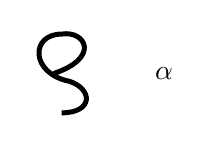
\begin{tikzpicture}[x=1cm,y=1cm]
\draw[line width=1.8pt] (0,.1) .. controls (.6,.3) and (.4,.65) .. (.1,.6) .. controls (-.3,.6) and (-.3,.1) .. (.2,0) .. controls (.5,-.1) and (.5,-.4) .. (.1,-.4);
\node at (1.4,.1) {$\unsure{\alpha}$};
\end{tikzpicture}}
\diagram{\begin{tikzcd}
\widehat A\widehat\otimes\widehat A & \widehat A\arrow[l]
\end{tikzcd}}
\[
\boxed{(\widehat A(\Sigma,\Sigma_+,t))^{k'}=\widehat A_*(\Sigma^{k'},\Sigma_+^{k'},t^{k'})}
\]
\[
\widehat A_*(S,S_+,t)
\]
\[
(A^*(\Sigma,\Sigma_+,t))^\vee=\widehat A_*(\Sigma^\vee,\Sigma_+^\vee,t^\vee)
\]
\figure{\begin{tikzpicture}[x=1cm,y=1cm]
\draw (-4,1.3) .. controls (-5,1) and (-5,-1.2) .. (-3.8,-1.6) .. controls (-1,-2) and (3.8,-1.8) .. (4.3,-.9) .. controls (4.8,.6) and (4.3,1.5) .. (2.9,1.6) .. controls (.4,1.9) and (-3,1.7) .. (-4,1.3);
\node at (-3.7,1.8) {$\Sigma/k$};
\node at (-4.9,.7) {$\deleted{\unsure{R}}$};
\node at (-3.7,.15) {$\begin{array}{c}\Sigma^{\unsure{k'}}\\\bigcup\\\deleted{k}\\\Sigma'\end{array}$};
\draw (-2.9,1.1)--(-2.9,-1.2);
\node[align=left] at (.6,.8) {\(\text{(coalgèbre }\deleted{\unsure{graduée}}\inserted{\unsure{donnée|divisée}}\text{ avec sous-coalgèbre}\)};
\node[align=left] at (.6,.2) {et \unsure{copuiss. divisées} \uline{\unsure{respect celle-ci}}};
\node[align=left] at (.6,-.45) {\unsure{enfin on donne}\quad\(\Sigma\xrightarrow{t}k\)};
\node[align=left] at (.1,-1) {nulle sur \(\deleted{\unsure{k}}\Sigma'\)};
\end{tikzpicture}}
\diagram{\begin{tikzcd}
& t_k\arrow[d,phantom,"{\rotatebox{-90}{\(\unsure{\in|\simeq}\)}}" description] &&\\
0\arrow[r] & \boxed{\unsure{\mathbb Z|Z}}^{k+}\arrow[r] & \underbrace{\Sigma^k}_{\unsure{\text{anneau}}}\arrow[r,nohead] & \Sigma'{}^k\\
& \text{idéal} && \unsure{\text{anneau}}
\end{tikzcd}}
\[
k\{\{T\}\}\{\{\gamma_0,-\gamma_-\}\}
\]
}
\mspage{281}
